%\documentclass[iop,twocolumn, tighten, twocolappendix, numberedappendix]{emulateapj}
%\documentclass[iop,onecolumn]{revtex4-1}
%\documentclass[rmp,aps,twocolumn]{revtex4-1}
\documentclass[rmp,aps]{revtex4-1}

\usepackage[backref,breaklinks,colorlinks,citecolor=blue]{hyperref}  
\usepackage[all]{hypcap}
\renewcommand*{\backref}[1]{[#1]}
\newcommand{\x}{\sout}


\usepackage{amsmath}
\usepackage{amssymb}
\usepackage{graphicx}
\usepackage{color}
\usepackage{natbib}
\usepackage{xspace}
\usepackage{nicefrac}
\bibliographystyle{hapj}
\usepackage[dvipsnames]{xcolor}
\newcommand\myshade{85}
\usepackage[T1]{fontenc}
\usepackage{lmodern}
\usepackage{tablefootnote}
\usepackage{ulem}
\usepackage{floatflt}
\usepackage{wrapfig}
 	
\colorlet{mycitecolor}{Turquoise}
\colorlet{mylinkcolor}{Turquoise}

\hypersetup{
 citecolor = mycitecolor!\myshade!black,
 linkcolor = mylinkcolor!\myshade!black,
 colorlinks = true,
}

\def\aj{Astronomical Journal}             % Astronomical Journal
\def\apj{Astrophysical Journal}                % Astrophysical Journal
\def\apjl{Astrophysical Journal}             % Astrophysical Journal, Letters
\def\pasj{PASJ}
\def\apjs{ApJS}              % Astrophysical Journal, Supplement
\def\mnras{MNRAS}            % Monthly Notices of the RAS
\def\prd{Phys.~Rev.~D}       % Physical Review D
\def\prl{Phys.~Rev.~Lett}    % Physical Review Letters
\def\cqg{Class.~Quant.~Grav.~}%Classical and Quantum Gravity
\def\araa{ARA\&A}             % Annual Review of Astron and Astrophys
\def\nat{Nature}              % Nature
\def\aap{A\&A}                % Astronomy and Astrophysics
\def\na{New Astronomy}
\def\nar{New Astronomy Reviews}
\def\pasa{Publications of the Astron.~Soc.~of Australia}
\def\aapr{Astron.~\& Astrophys.~Reviews}
\def\physrep{Physics Reports}
\def\apss{Ap\&SS}


\newcommand{\todo}[1]{\textcolor{red}{#1}}
\newcommand{\tocheck}[1]{\textcolor{green}{Check: #1}}
\newcommand{\citeme}{{\color{magenta} CITE ME!}}
\newcommand{\ajf}[1]{\textcolor{red}{#1}}
%\newcommand{\ilya}[1]{\textcolor{magenta}{#1}}
\newcommand{\ilya}[1]{\textcolor{magenta}{\bf{#1}}}

\def\be{\begin{equation}}
\def\ee{\end{equation}}
\def\ba{\begin{eqnarray}}
\def\ea{\end{eqnarray}}
\def\rsquo{'}


%\submitted{Submitted \today}

\begin{document}

\title{Merging stellar-mass binary black holes}
%\shorttitle{}

\def\addBham{Institute of Gravitational Wave Astronomy and School of Physics and Astronomy, University of Birmingham, Edgbaston, Birmingham B15 2TT, United Kingdom}
\def\addMonash{Monash Centre for Astrophysics, School of Physics and Astronomy, Monash University, Clayton, Victoria 3800, Australia}


\author{Ilya Mandel}
\email{imandel@star.sr.bham.ac.uk}
\affiliation{\addBham\\ and\\ \addMonash}
\author{Alison Farmer}
\affiliation{kW Engineering, Oakland, California, 94612, USA}

\begin{abstract}

The LIGO and Virgo detectors have recently directly observed gravitational waves from several mergers of pairs of stellar-mass black holes, as well as from one merging pair of neutron stars.  These observations raise the hope that compact object mergers could be used as a probe of stellar and binary evolution, and perhaps of stellar dynamics. This colloquium-style article summarizes the existing observations, describes theoretical predictions for formation channels of merging stellar-mass black-hole binaries along with their rates and observable properties, and presents some of the prospects for gravitational-wave astronomy.

\end{abstract}

\maketitle

\section{Introduction}

\ilya{Our goal is to present an informal, colloquium-style article on the subject of} merging stellar-mass black-hole binaries as gravitational-wave sources. Several reviews were written in the excitement following the first detection \citep{GW150914} of gravitational waves by the Laser Interferometer Gravitational-wave Observatory (LIGO) \citep{GW150914:detectors}, including the astrophysical context companion paper by the the LIGO-Virgo scientific collaboration \citep{GW150914:astro} and the excellent article by \citet{Miller:2016}. However, it is somewhat premature to formally review a field that is both rapidly evolving and very much in its infancy.  With just a few detections to date of gravitational waves from merging black holes \citep{GW150914,GW151226,BBH:O1,GW170104,GW170608,GW170814}, and one from merging neutron stars \citep{GW170817}, we are only beginning to explore the population of merging compact-object binaries.  \ilya{The understanding of the formation channels for these sources is evolving with each new detection.} 
%We are not yet certain even of the dominant formation channels for these sources; \ilya{our

The full range of astrophysical questions that gravitational-wave observations will answer is itself a topic of active study and debate. \ilya{For example:} What can gravitational-wave observations of merging binaries tell us about the stellar and binary evolution that preceded the mergers?  Can the observations constrain the amount of mass loss and expansion experienced by massive stars? Or the stability and consequences of mass transfer, including the infamous common-envelope phase of evolution? Or the amount of mass fallback during supernova explosions, or the kicks that supernovae impart to compact objects? Does the redshift distribution of merging compact objects contain an imprint of the star formation history of the Universe?  Can we use these mergers to probe dynamics in dense stellar environments such as globular clusters? The answers to these important and exciting questions may also in turn influence our understanding of topics as diverse as reionization and heavy-element nucleosynthesis.

In this article, we focus on the questions that strike us as being most interesting and timely at this stage of the field's development.  The choice of these questions is undoubtedly biased by our own interests. Further, we do not attempt to systematically survey all of the relevant literature.  In other words, this is emphatically {\it not} a review \citep{magritte}. 

We summarize the existing observations of merging binary black holes and closely related systems in \autoref{obs}, describe the plausible formation scenarios for binary black holes in \autoref{form}, discuss the predicted merger rates and merging object properties in \autoref{merge}, and speculate about the prospects for gravitational-wave astronomy in \autoref{prospect}.


 

\section{Observations}\label{obs}

\subsection{Gravitational-wave observations}


\subsubsection{The confirmed detections to date}
During its first observing run, lasting from September of 2015 through January of 2016, the \ilya{advanced} LIGO detector network observed three likely signals from the mergers of binary black holes.  GW150914 \citep{GW150914} and GW151226 \citep{GW151226} were confident, $> 5\sigma$ observations; LVT151012 was estimated as having a $\sim 90\%$ probability of being a gravitational-wave signal \citep{GW150914:rates,BBH:O1}, though the estimate is conservative and we shall treat it as a detection here.  During the second observing run, lasting with some interruptions from November 2016 through August 2017, three further confident binary black hole detections were announced: GW170104 \citep{GW170104},  GW170608 \citep{GW170608}, and GW170814 \citep{GW170814}, the last of these with the participation of the Virgo gravitational-wave observatory \citep{AdvVirgo}.   The observation of gravitational waves from the binary neutron star merger GW170817 \citep{GW170817} was followed up by an unprecedented campaign of electromagnetic observations, leading to detections of a short gamma ray burst, optical kilonova, and an afterglow spanning from radio through X-ray wavelengths \citep{GW170817:GRB,GW170817:MMA}.  We shall focus on binary black holes for the remainder of this article.

\subsubsection{Information encoded in gravitational-wave signals}
The gravitational-wave signature encodes the properties of the merging binary black holes: the component masses and spins. Coupled with information from two or more detectors in a network, this makes it possible to infer the sky location and orientation of the source and the distance to the source \citep{Veitch:2014,GW150914:PE}.  However, some of the source parameters are strongly correlated, leading to near-degeneracies when attempting to extract them from a noisy dataset.   For the heaviest black\ilya{-}hole binaries such as GW150914, the total mass $M \equiv M_1 + M_2$ is measured relatively accurately because the latest stage of the merger waveform, the ringdown, whose frequency is a function of the total mass, falls in the sensitive frequency band of current gravitational-wave detectors.  For most black-hole binaries, the chirp mass $M_c \equiv M_1^{3/5} M_2^{3/5} M^{-1/5}$ is the better measured parameter, since it determines to lowest order the rate of frequency evolution during the earlier inspiral phase of the waveform.  The mass ratio $q\equiv M_2/M_1 \leq 1$ is often quite poorly constrained, because it enters the gravitational-wave phase evolution during inspiral at a higher order in the ratio of the orbital velocity to the speed of light and is partially degenerate with the black\ilya{-}hole spins \citep[e.g.,][]{PoissonWill:1995}.  

\subsubsection{Information extracted from the observed gravitational-wave signals}
We list the parameters of the black\ilya{-}hole binaries observed to date in table \ref{table:BHmasses}. Specific system properties are discussed below.

\begin{table}
\begin{tabular}{lcccccc}
Event  & $M_c$ [$M_\odot$]  & $q$ & $M_1$ [$M_\odot$]  & $M_2$ [$M_\odot$]  & $\chi_\textrm{eff}$ & $d_L$ [Mpc] \\
\hline
GW150914\footnote{\citet{BBH:O1}} & $28.1^{+1.8}_{-1.5}$ & $0.81^{+0.17}_{-0.2}$ & $36.2^{+5.2}_{-3.8}$ & $29.1^{+3.7}_{-4.4}$ & $-0.06^{+0.14}_{-0.14}$ & $420^{+150}_{-180}$\\
LVT151012$^\mathrm{a}$ & $15.1^{+1.4}_{-1.1}$ &$0.57^{+0.38}_{-0.37}$ &$23^{+18}_{-6}$ &$13^{+4}_{-5}$ &$0.03^{+0.31}_{-0.20}$ &$1020^{+500}_{-490}$\\
GW151226$^\mathrm{a}$ & $8.88^{+0.33}_{-0.28}$ &$0.52^{+0.40}_{-0.29}$ &$14.2^{+8.3}_{-3.7}$ &$7.5^{+2.3}_{-2.3}$ &$0.21^{+0.20}_{-0.10}$ &$440^{+180}_{-190}$ \\
GW170104\footnote{\citet{GW170104}} & $25.1^{+2.5}_{-3.9}$ &$0.62^{+0.32}_{-0.26}$ &$31.2^{+8.4}_{-6.0}$ &$19.4^{+5.3}_{-5.9}$ &$-0.12^{+0.21}_{-0.30}$ &$880^{+450}_{-390}$\\
GW170608\footnote{\citet{GW170608}} & $7.9^{+0.2}_{-0.2}$ &$0.6^{+0.3}_{-0.4}$ &$12^{+7}_{-2}$ &$7^{+2}_{-2}$ &$0.07^{+0.23}_{-0.09}$ &$340^{+140}_{-140}$ \\
GW170814\footnote{\citet{GW170814}} & $24.1^{+1.4}_{-1.1}$ & &$30.5^{+5.7}_{-3.0}$ &$25.3^{+2.8}_{-4.2}$ &$0.06^{+0.12}_{-0.12}$ & $540^{+130}_{-210}$ \\
\hline
\end{tabular}
\caption{The parameters of merging binary black holes inferred from gravitational-wave observations: chirp mass $M_c$, mass ratio $q=M_2/M_1$, component masses $M_1$ and $M_2$, effective spin $\chi_\textrm{eff}$, and luminosity distance $d_L$.  The median value and the 90\% credible interval bounds are given.}\label{table:BHmasses}
\end{table}

\textbf{Masses:} The individual black\ilya{-}hole masses span a range from $\ilya{\simeq} 7 M_\odot$ to $\ilya{\simeq} 35 M_\odot$.  The masses appear to be roughly uniformly distributed over this range.  However, there is a significant selection bias  toward detecting more massive systems, because sensitivity to gravitational waves from binary mergers depends on the system mass.  The gravitational-wave amplitude, and hence the maximum (horizon) distance at which a source is detectable, scales as $M_c^{5/6}$ for inspiral-dominated signals. The surveyed volume therefore scales as $M_c^{2.5}$.  While the existing observations are not sufficient to accurately determine the mass distribution of merging binary black holes, the observed broad mass distribution, deconvolved with the mass-dependent selection effects, could be consistent with an intrinsic mass distribution of \ilya{$M^{-2.3_{-1.4}^{+1.3}}$} \citep{BBH:O1,GW170104}, reminiscent of the stellar initial mass function \citep{Salpeter:1955}.  The uncertainty in the mass distribution is relayed into the uncertainty on inferred merger rates, which are consistent with a broad range spanning $\sim 10$ -- $200$ Gpc$^{-3}$ yr$^{-1}$ \citep{GW170104}.  

\textbf{Mass Ratios:} While all binary black holes observed to date are consistent with having equal-mass components, mass ratios could be as extreme as $4:1$ in some cases.  

\textbf{Black\ilya{-}Hole Spins:} Individual black\ilya{-}hole spins are difficult to measure precisely with gravitational waves.  However, we do know that none of the observed binaries could have large spins aligned with the orbital angular momentum; in fact the `effective spin' $\chi_\textrm{eff}$ --- the mass-weighted dimensionless spin along the direction of the orbital angular momentum --- is below $0.4$ for all observed events, and consistent with zero for all but one of them.  Interestingly, $\chi_\textrm{eff}$ is not consistent with zero for GW151226, the second lightest binary black hole detected, indicating that at least one of the components for that event must have been a rotating black hole.  Spin projections in the orbital plane are very poorly constrained for all events.

\textbf{Distances and Sky Locations:} All of the observed \ilya{binary black hole} signals came from distances of around 500 Mpc to 1 Gpc (redshifts $z\sim 0.1$ -- $0.2$), \ilya{consistent with the detector sensitivity during the first two observing runs of advanced LIGO}.  With just two operational detectors, LIGO Hanford and LIGO Livingston, for all events prior to GW170814, sources could only be localized to 90\% credible regions spanning hundreds to more than a thousand square degrees on the sky.  The participation of the Virgo instrument in the observation of GW170814 reduced the sky region to only 60 deg$^2$ \citep{GW170814}.  Nonetheless, associations with specific host galaxies are impossible for all observed binary black hole mergers.  

\textbf{Testing General Relativity:} All gravitational-wave signals observed to date are consistent with gravitational waves expected within the general theory of relativity, providing a stringent test of this theory in the dynamical, strong-field regime \citep{GW150914:GR,GW170104}.

\subsection{Electromagnetic observations}

While recent gravitational-wave observations have invigorated the field of massive binary evolution, there already exists a wealth of electromagnetic observations of systems at various stages along the possible paths to binary black hole formation. In this section we describe some of the key electromagnetic observations that shed light on compact object binary formation and evolution preceding \ilya{the} merger.

A wide variety of electromagnetic observations inform our understanding of the evolution of massive stellar binaries. These include observations of: 
\begin{itemize}
\item the initial mass and period distributions of binary stars at formation \citep[e.g.,][]{Sana:2012,MoeDiStefano:2017}; 
\item luminous red novae, which may be associated with common envelope events \citep[e.g.,][]{Ivanova:2013LRN};
\item Galactic binary radio pulsars \citep[e.g.,][]{Tauris:2017};
\item short gamma-ray bursts \citep[e.g.,][]{Berger:2014};
\item supernovae and long gamma-ray bursts \citep[e.g.,][]{Cantiello:2007,Szecsi:2017};
\item X-ray binaries \citep[e.g.,][]{TaurisvdH:2006}.
\end{itemize}
Here we focus on X-ray binaries, the type of binary system with the closest connection to merging binary black holes, although only a small minority of black-hole X-ray binaries will ultimately evolve into merging black holes \citep[e.g.,][]{CygnusX3:2012}. Black\ilya{-}hole X-ray binaries consist of a star transferring mass onto a black\ilya{-}hole companion, leading to the emission of X-ray radiation from the accretion disk surrounding the black hole. 

\subsubsection{X-ray binaries}

X-ray binaries containing accreting black holes can be divided into two categories, low-mass and high-mass, in reference to the mass of the black hole's companion star. The accretion process differs between the two types: in low-mass X-ray binaries, the tidal field of the black hole is causing mass to stream from the companion on to the black hole in the process known as Roche-lobe overflow, while in high-mass X-ray binaries, the black hole accretes only a fraction of the material (stellar wind) driven off the companion's surface.

\textbf{Black\ilya{-}Hole Masses:} 
Black-hole X-ray binaries with dynamical mass measurements provide the only secure measurements of black\ilya{-}hole masses other than the gravitational-wave observations described above.  \citet{Ozel:2010} and \citet{Farr:2011} summarize the mass distribution of black-hole X-ray binaries; they find a distribution which ranges from 4 or 5 solar masses for the lightest low-mass X-ray binaries (with a possible mass gap between neutron\ilya{-}star and black\ilya{-}hole masses) to \ilya{$\gtrsim 20\, M_\odot$} for the heaviest high-mass X-ray binaries.  However, given the doubts subsequently placed on the radial velocity measurements in high-mass X-ray binaries such as IC10 X-1 \citep{Laycock:2015}, there are no known black holes with dynamically confirmed masses certain to exceed \ilya{$\simeq 15\, M_\odot$}.  The measured masses of black holes in X-ray binaries are sketched in figure \ref{fig:BHmasses}, along with the masses of the observed gravitational-wave sources.  This figure does not include the speculative but potentially very exciting evidence for intermediate-mass black holes \citep{MillerColbert:2004,Pasham:2014}; if such few-hundred solar-mass black holes generically exist in globular clusters, they will \ilya{substitute into merging binaries and ultimately be observable} as gravitational-wave sources \citep[e.g.,][]{Mandel:2008,IMBBH:O1}.

\begin{figure}
	\centering
	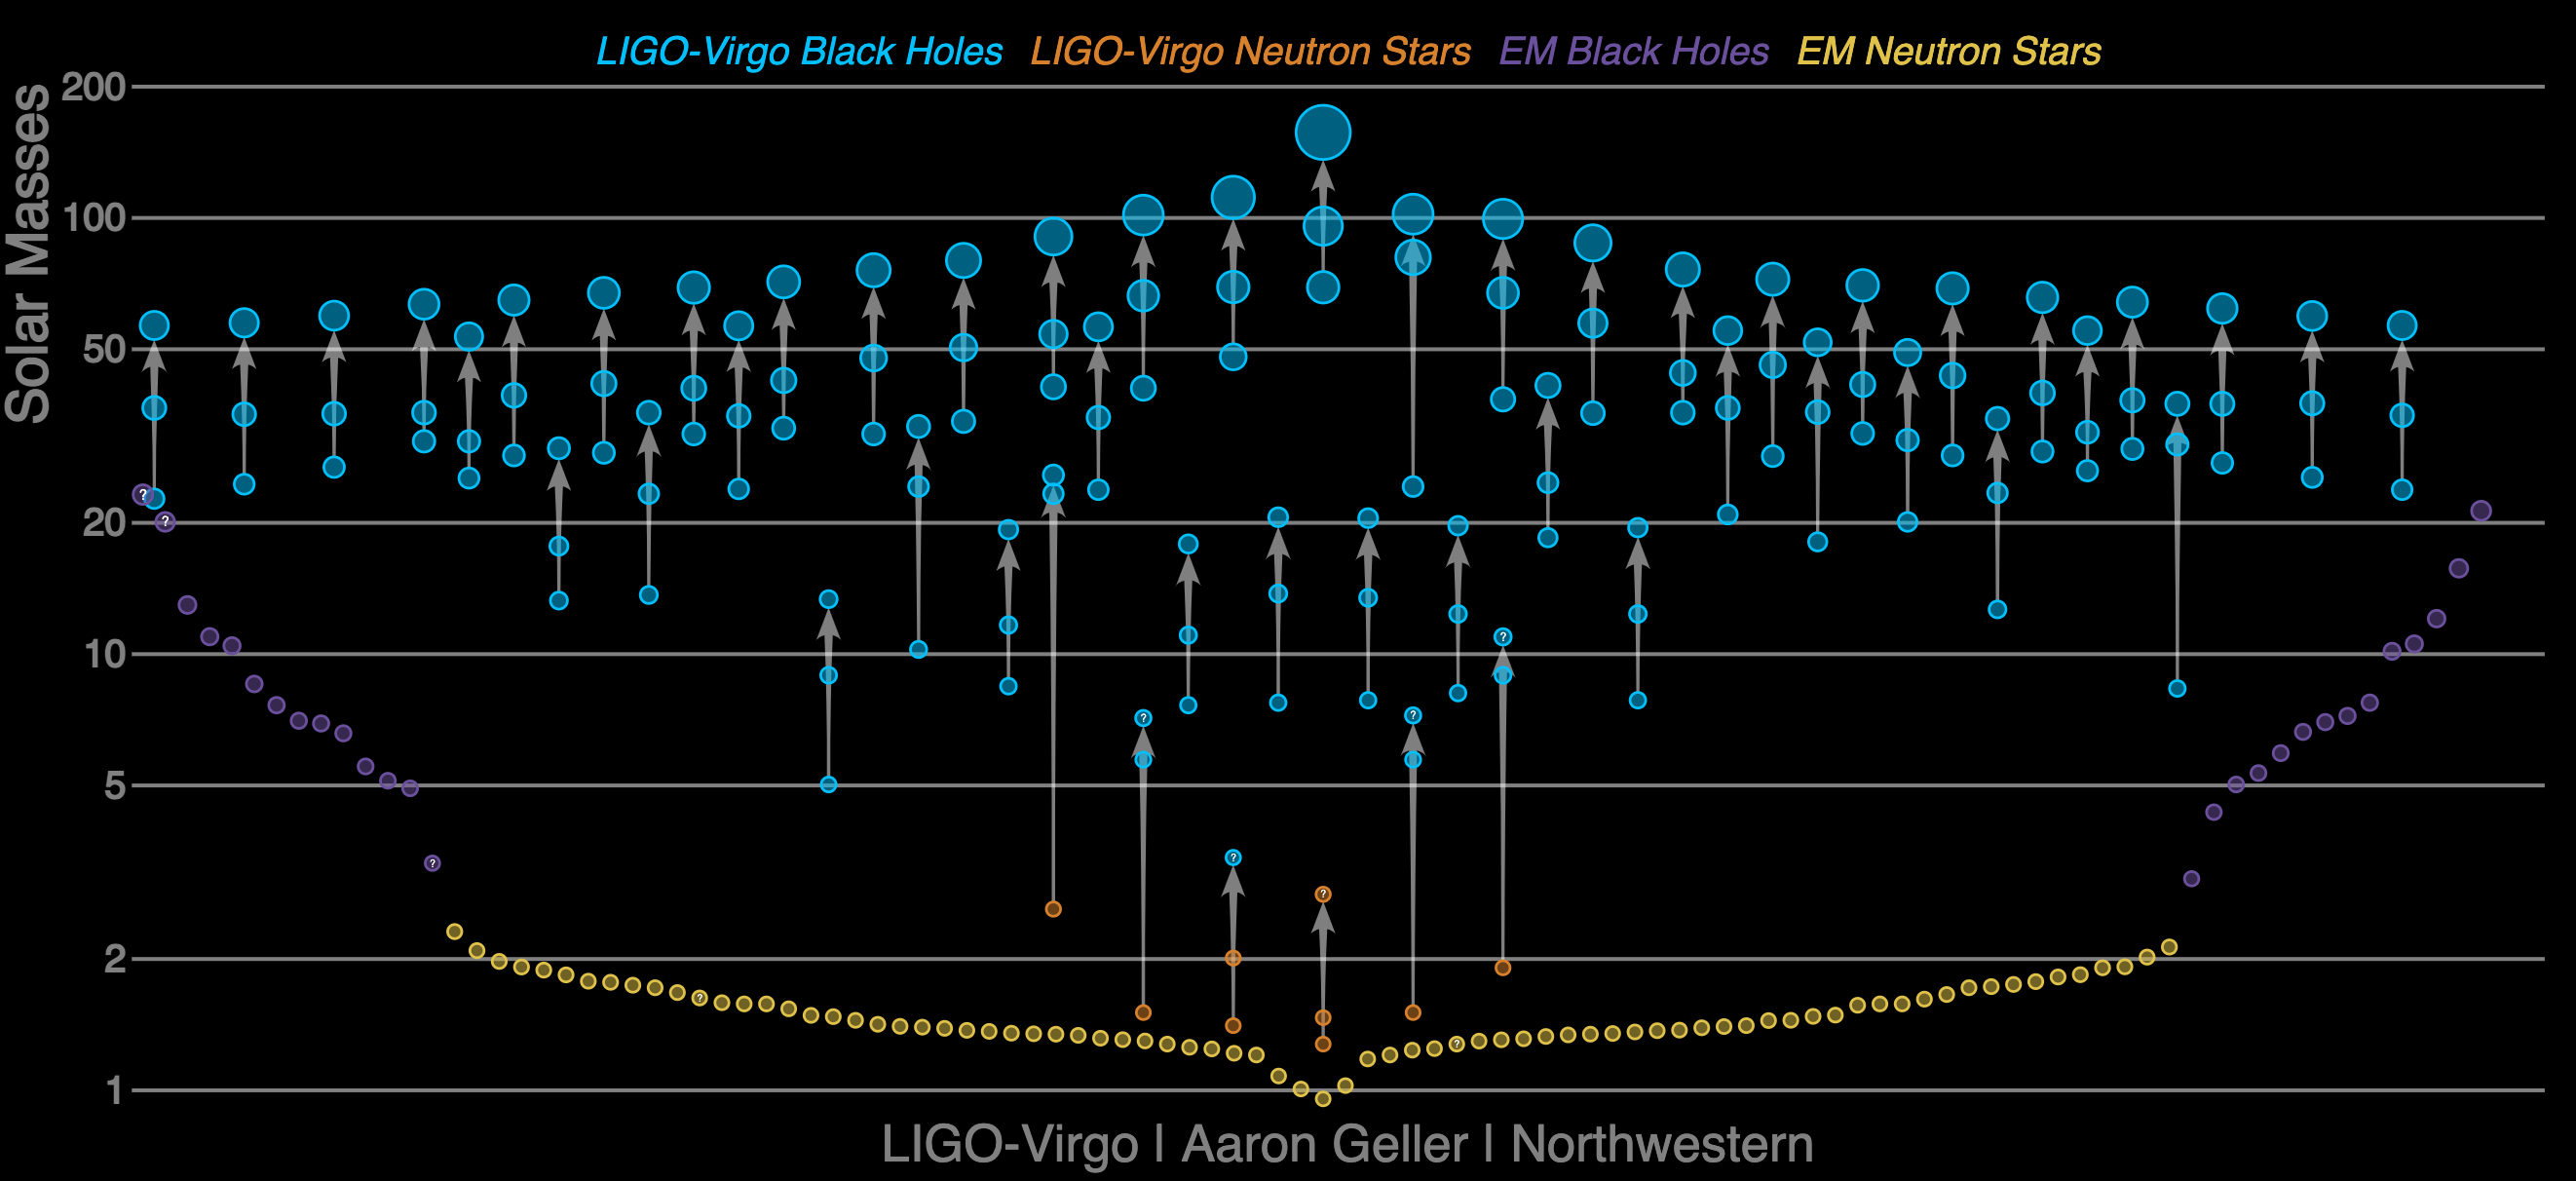
\includegraphics[width=0.99\textwidth]{Graveyard.png}
	\caption{\label{fig:BHmasses}  The masses (in solar masses, vertical axis) of black holes observed as gravitational-wave sources (blue), as well as masses of black holes in X-ray binaries (purple).  Galactic neutron stars observed as radio pulsars (yellow) and the merging double neutron star GW170817 (orange) appear at the bottom of the figure.  Merger product masses are shown for gravitational-wave detections. Placement on the horizontal axis is arbitrary.  Error bars are indicative of the measurement uncertainty.  Figure courtesy of Frank Elavsky, Northwestern University and LIGO-Virgo collaborations.}
\end{figure}


\textbf{Black\ilya{-}Hole Spin Magnitudes:} Black\ilya{-}hole X-ray binaries also provide an opportunity for measuring 
	black\ilya{-}hole spins \citep[see][for a recent review]{MillerMiller:2015}.  Continuum fitting of the X-ray flux from the accretion disk and iron K-$\alpha$ line fits to the disk reflection profile can both be used to infer the location of the inner edge of the disk, which is assumed to correspond to the radius of the innermost stable circular orbit, a sensitive function of black\ilya{-}hole spin.  Quasi-periodic oscillations also have the potential to provide spin measurements.  Unfortunately, the underlying physical mechanisms are not fully understood at present, and the inferred spins may suffer from significant systematics.  For example, out of six systems for which both disk continuum and disk reflection spin measurements are available, the two methods are inconsistent at the $3$ or $5$ sigma level for two systems, and for one system the statistical uncertainty is so large as to span nearly the full allowed range from $0$ to $1$ \ilya{\cite{MillerMiller:2015}}.  However, for the remaining three systems with both measurements available, both methods yield spins $\chi \gtrsim 0.9$.  

\textbf{Inconsistency with Spin Observations from Gravitational-wave Sources?} These \ilya{three} high-spin observations include two high-mass X-ray binaries: LMC X-1 and Cygnus X-1.  This is significant, because unlike long-lived low-mass X-ray binaries, whose spin magnitudes could be altered by accretion from the companion, especially if they started out with intermediate-mass companions \citep{Podsiadlowski:2003,Fragos:2015}, high-mass X-ray binaries are too short-lived to enable significant spin changes due to accretion \citep{KingKolb:1999}.  Isolated binaries that form binary black holes are expected to go through the high-mass X-ray binary phase during their evolution.  Thus, if the high spin magnitude measurements in black-hole X-ray binaries are to be believed, then either some future merging binary black holes should be observed to have high spins like those in X-ray binaries, or, perhaps more likely, the observed high-mass X-ray binaries and merging binary black holes sample different evolutionary histories (see \autoref{BHspins}).

\textbf{Black\ilya{-}Hole Spin Directions:} We know even less about the spin directions than the spin magnitudes.  Although black-hole spin-orbit alignment is assumed in continuum flux measurements \citep{MillerMiller:2015}, some black-hole X-ray binaries, including GRO J1655-40 \citep{Martin:2008}, 4U 1543-47 \citep{MorningstarMiller:2014} and particularly V4641 Sgr \citep{Orosz:2001,Martin:2008b} appear to indicate that the microquasar jet, presumably aligned with the BH spin axis, is misaligned with the orbit.  Moreover, initial stellar spins in binaries have been observed to be misaligned \citep[e.g.,][]{Albrecht:2009,Albrecht:2014}, though there are opportunities for realignment during binary evolution, as described below.

\section{Formation scenarios}\label{form}

When the detection of GW150914 was first announced, many were surprised that it was a binary black hole rather than a binary neutron star: there was already observational evidence for merging double neutron stars in the Galaxy (starting with the Hulse-Taylor binary pulsar \citep{HulseTaylor:1975}), but there was no direct evidence for merging binary black holes. Some were even more surprised by the high black\ilya{-}hole masses, in excess of the observed black\ilya{-}hole masses in X-ray binaries. Was this surprise justified? And should we be perplexed by the spin or mass ratio measurements for the gravitational-wave sources? Before answering these questions, we should first discuss how these merging compact binaries come into existence. In fact, this is one of the key outstanding questions that gravitational-wave observations will help us to answer. Below, we explain why -- on the face of it -- it is rather startling that compact massive binaries exist at all. We then describe the leading candidate formation channels, and in the next section we discuss the ways in which gravitational-wave observations might be used to distinguish them.


\subsection{The \ilya{Orbital} Separation Question}


\textbf{Only very tight binaries can merge via gravitational waves.} Gravitational-wave emission is a very strong function of separation. During a compact binary merger, the luminosity in gravitational waves is a few thousandths of the Planck luminosity, $c^5/G$ \citep[e.g.,][]{Cardoso:2018}; at nearly $10^{57}$ ergs per second, such mergers ``outshine'' all the stars in the visible Universe combined. But because gravitational-wave luminosity is inversely proportional to the fifth power of the binary separation \citep{Peters:1964}, widely separated binaries lose energy very slowly and undergo only negligible inspiral over billions of years. Only very close binaries can be brought to merger by gravitational waves within the age of the universe; \autoref{fig:periapsis} shows the maximum initial separation for an equal-mass binary to merge on this timescale. For the two \ilya{$\sim 30 M_\odot$} black holes responsible for GW150914, the initial separation must have been less than $\sim 50 R_\odot$ -- just a quarter of the distance from the Earth to the Sun -- if the merger was driven by gravitational-wave emission alone.


\textbf{But the black holes' parent stars \ilya{cannot} get so close.} Stars expand as they evolve. Even our Sun will reach roughly an astronomical unit in size during its giant phase; the stars (above $\sim 20 M_\odot$  at birth) that leave behind black holes may reach thousands of solar radii at their maximal extent. The maximum stellar radius as a function of initial mass is plotted in \autoref{fig:Rmax}. \ilya{There appears to be} a problem. If the parent stars begin life at separations from which gravitational waves could bring their remnants together, the stars will expand to sizes larger than their separation as they evolve, and we might therefore expect that they would merge long before they collapse into black holes. If they start sufficiently far apart to avoid merger before collapse, their remnant binaries will take many millions of times the age of the universe to merge. In either case, no gravitational-wave sources would exist today. 

\textbf{The problem is already there at birth.} In fact, for reasonable models of wind-driven mass loss and mass loss during supernovae, even the initial stellar radii at the start of the main sequence are too large to fit into a binary that could merge within the age of the Universe just through gravitational-wave emission.  The black `Roche Lobe' curve in \autoref{fig:Rmax} shows the maximum size that a star could have in order to fit into a circular, merging equal-mass binary (see \autoref{fig:periapsis}).  This size is smaller than the zero-age main sequence radius for all stellar masses shown in the figure: the separation problem thus exists even without accounting for the exacerbating factors of stellar expansion or binary widening through mass loss.


\begin{figure}
	\centering
	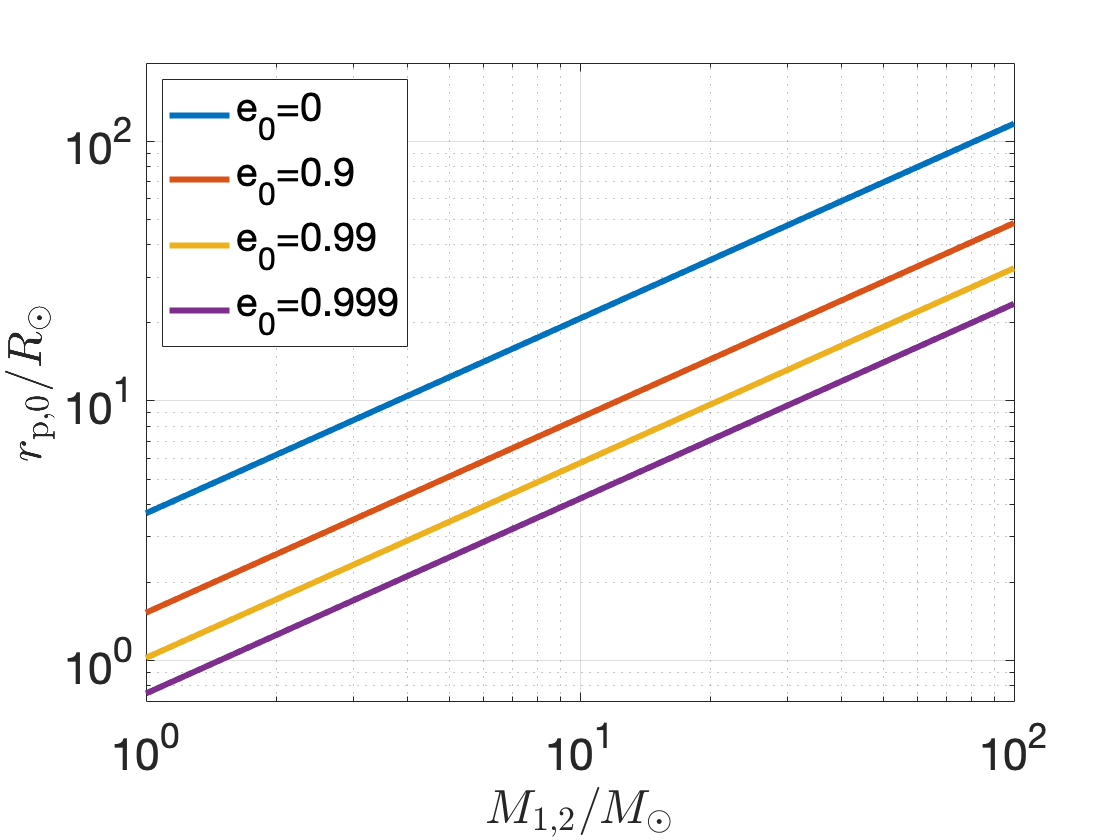
\includegraphics[width=0.5\textwidth]{M-rp-log.png}
	\caption{Maximum initial periapsis separation that a binary black hole with equal-mass components (as given on the ordinate) can have while still merging within the age of the Universe through gravitational-wave emission, for four different choices of initial eccentricity: $e=0$, 0.9, 0.99, and 0.999 from the top down.\label{fig:periapsis}}
\end{figure}
	
\begin{figure}
	\centering	
	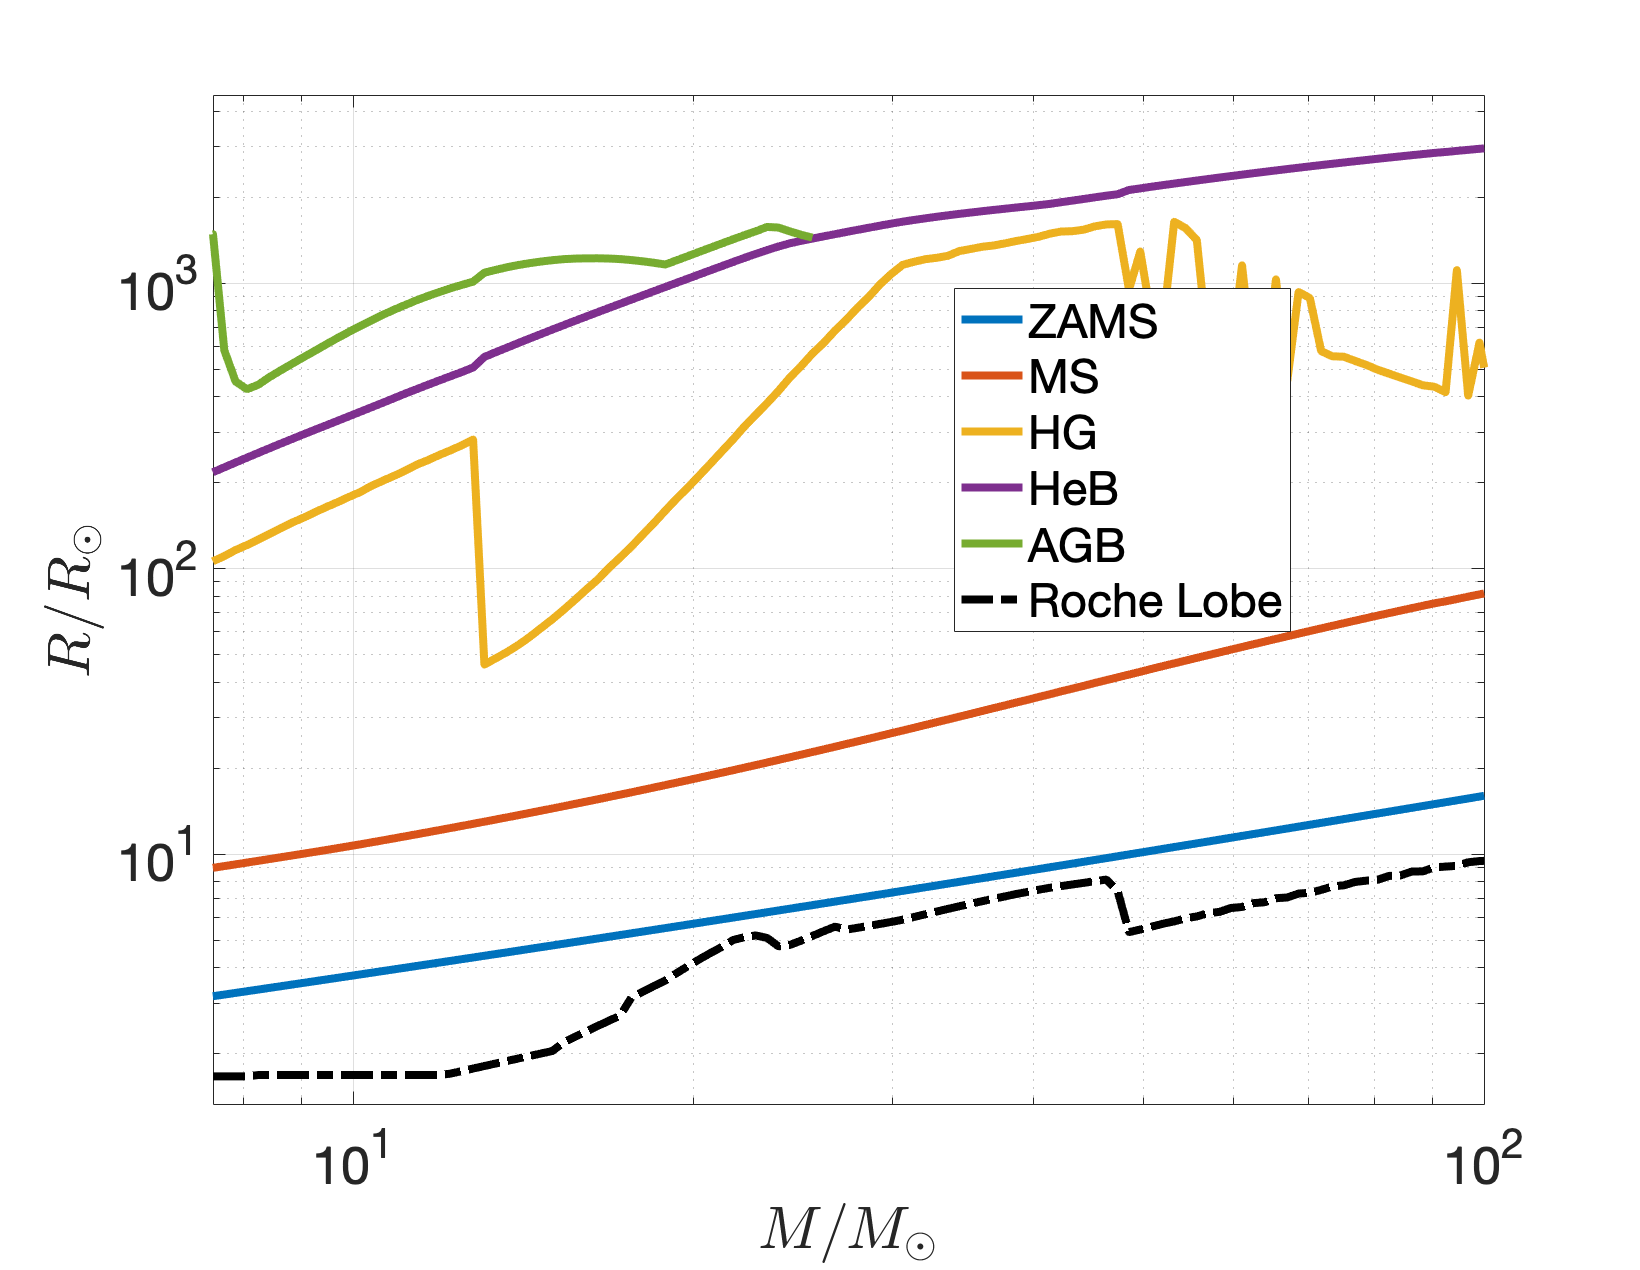
\includegraphics[width=0.5\textwidth]{StellarRadiusZsolarRoche.png}
\caption{Maximal stellar extent at solar metallicity during various phases of stellar evolution for a non-rotating star with a given initial mass; based on the implementation of single stellar evolution models of \citet{Hurley:2000} in the COMPAS binary population synthesis code \citep{Stevenson:2017}.   The star expands from its zero-age main sequence (ZAMS) size onwards through the main sequence (MS), Hertzsprung gap (HG), core Helium burning (CHeB) stages, and the asymptotic giant branch (AGB) for lower-mass stars.  The Roche lobe radius (maximal stellar size beyond which a star would engage in mass transfer \citep{Eggleton:1983}) is plotted for an equal mass circular binary which would have the maximum separation to allow a merger within the age of the Universe (see \autoref{fig:periapsis}) assuming initial mass to compact object mass conversion as in \autoref{fig:BHremnant}.\label{fig:Rmax} }
\end{figure}

\textbf{So then why do the gravitational-wave sources exist at all?} Given the above, one might conclude that gravitational-wave driven compact binary mergers do not exist. Yet their existence and detection were expected \citep{ratesdoc}. In fact, \citet{Dyson:1962} conjectured about the existence of merging neutron star binaries even before the first neutron star was observed; \citet{Tutukov:1973} predicted that binary compact objects must naturally (albeit rarely, and at wide separations in their model) form as a result of massive binary evolution; \citet{vdHDeLoore:1973} argued that tight high-mass X-ray binaries -- progenitors of compact object binaries -- must also form; and the Hulse--Taylor binary pulsar \citep{HulseTaylor:1975} demonstrated the existence of binary compact objects that would merge within the age of the Universe \citep[for early explanations of its formation in the context of binary evolution, see][]{FlanneryvdH:1975,DeLoore:1975}.

Three leading formation scenarios have been proposed for merging compact-object binaries: (i) finely tuned binary evolution that brings the stars closer as they expand and interact; (ii) finely tuned stellar evolution that prevents the parent stars from expanding at all; and (iii) assembly of a close binary from black holes that formed from stars not born in the same binary. Contrived as these scenarios sound, all three might plausibly contribute to the production of binary black hole mergers.  And as we'll see in \autoref{merge}, only a small fraction of stars, of order one in a million, need to end up in merging black\ilya{-}hole binaries in order to explain the observed merger rates: even quite unusual or (apparently) finely tuned evolutionary pathways could therefore be viable candidates.

We explore the three leading formation scenarios in more detail below, as well as the possibility that some combination of these effects may occur on the way to merger. We won't discuss some of the more exotic proposed mechanisms, such as the fragmentation of a single stellar core into two black holes \citep{Loeb:2016} \ilya{(\citet{Woosley:2016} and \citet{Dai:2017} discuss the problems with this picture)} or non-astrophysical formation scenarios such as primordial black holes of cosmological origin \citep[e.g.,][]{Bird:2016}.

\subsection{The Candidate Formation Scenarios}
\subsubsection{Coming closer later in life: classical isolated binary evolution via the common-envelope phase}
\label{form:isol}

The first possible channel is perhaps the most studied one, placing merging black\ilya{-}hole binaries in the same framework as other very close binaries (such as cataclysmic variables) in which at least one of the stars has extended beyond the binary's current orbital separation during an earlier stage of its evolution \citep[e.g.,][]{Paczynski:1976}. 

In this scenario the two stars are born in a relatively wide binary, allowing them space to expand.  However, at a critical moment in its evolution, the binary is tightened by a factor of two or more orders of magnitude through dynamically unstable mass transfer, known as a common envelope phase; see \citet{Ivanova:2013} for a review. The resulting tight binary may then be close enough to merge through gravitational-wave emission.  \citet{SmarrBlandford:1976} may have been the first to explicitly point to this channel in the context of compact object binary formation when analyzing the evolutionary history of the Hulse--Taylor binary pulsar. The channel has been studied at length over the past 40 years, with significant contributions from \citet{TutukovYungelson:1993,Lipunov:1997,BetheBrown:1998,Nelemans:2003,VossTauris:2003,Pfahl:2005,Dewi:2006,Kalogera:2007,OShaughnessy:2008,Dominik:2012,Belczynski:2016,EldridgeStanway:2016} and many others. Rather than summarizing all of the steps and challenges in our understanding of massive binary evolution (see the papers above and the review by \citet{PostnovYungelson:2014} for details), we provide a schematic outline of an evolutionary scenario that leads to the formation of a GW150914-like merging system.

\begin{figure}
	\centering
	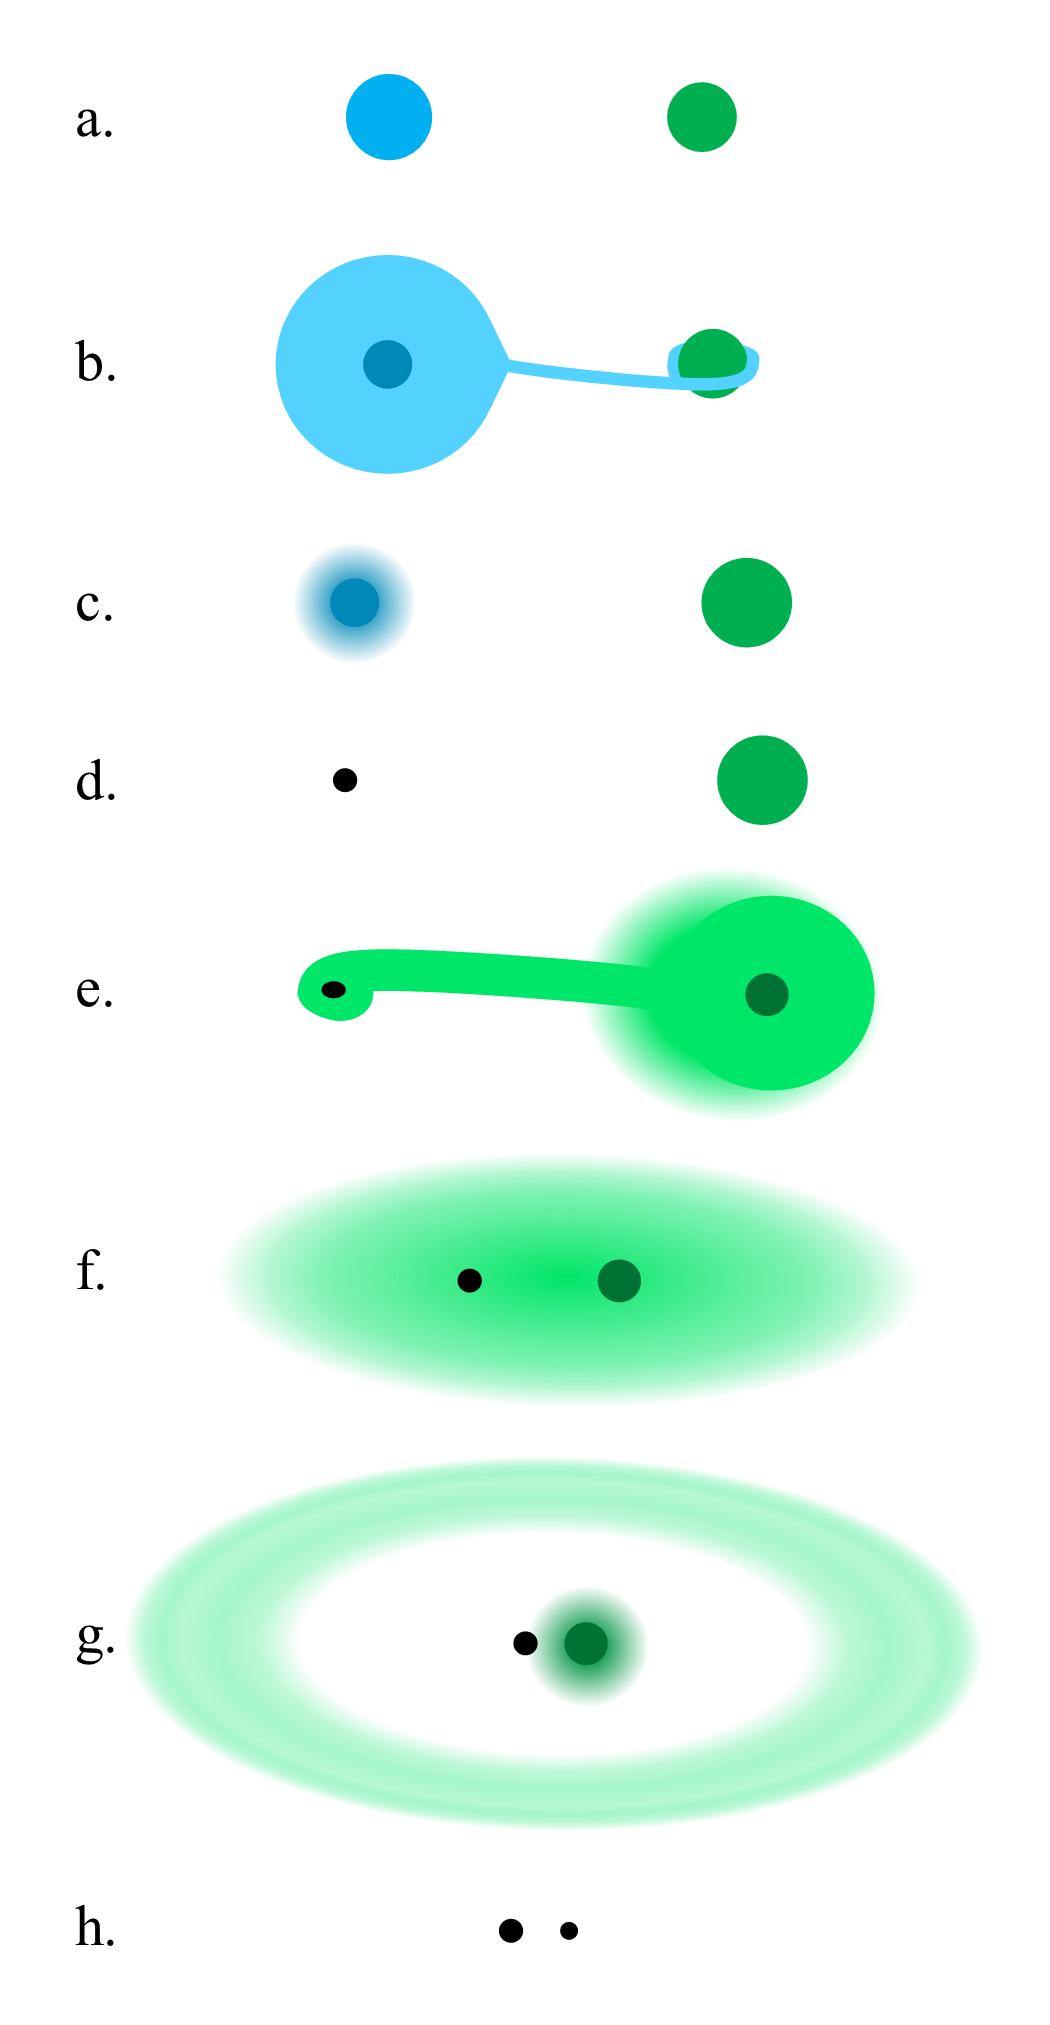
\includegraphics[width=0.45\textwidth]{channel1.png}
	\caption{\label{fig:isol_binary} A sketch of merging black\ilya{-}hole binary formation through isolated binary evolution via the common envelope phase.}
\end{figure}

\ilya{An example of the} evolution of this system is sketched out in a van den Heuvel -- style diagram in \autoref{fig:isol_binary}, and the steps below follow the panels in that figure:
\begin{enumerate}  
\item[a.] Two massive stars of perhaps $100$ and $75$ $M_{\odot}$ are born in a low-metallicity environment ($\sim 5\%$ of solar metallicity)  binary at a separation of $\sim 10$ AU.  
\item[b.] The more massive primary reaches the end of its main sequence evolution first.  At this stage, it has completed fusing hydrogen into helium in its core, and with the loss of energy input, the core begins to contract.  The associated release of gravitational binding energy and the eventual onset of hydrogen shell burning cause the hydrogen-rich envelope to expand.  For a sufficiently close binary, the primary expands past the equipotential surface known as the Roche Lobe and begins to transfer mass on to the secondary.  The mass transfer proceeds on the thermal timescale of the primary donor and could be significantly non-conservative, as the less evolved secondary, with its correspondingly longer thermal timescale, is unable to accept mass at the rate at which it is being donated.  The loss of mass from the binary, in addition to wind-driven mass loss, can widen the system to perhaps $\sim 20$ AU.  
\item[c.] The primary loses its entire envelope, leaving behind a naked helium-burning star -- a Wolf-Rayet star.  
\item[d.] Following wind-driven mass loss, which further widens the system, the primary collapses into a black hole; here, this collapse is assumed to be complete, without an associated natal kick.  
\item[e.] When, a few hundred thousand years later, the secondary reaches the end of its main sequence, the process repeats in reverse: the secondary expands until it commences mass transfer onto the primary.  By this time, the primary has lost around two thirds of its initial mass through a combination of envelope stripping, winds, and possible mass loss during a supernova (if the fallback is not complete).  The mass transfer on to the black hole would need to be almost wholly non-conservative if the accretion obeys the Eddington limit, which corresponds to an equilibrium between gravity and the pressure on infalling material of the radiation released during accretion.  Consequently, mass transfer would lead to a rapid hardening of the binary at a rate that is faster than the reduction in the size of the secondary donor as it loses mass.  As a result, the more mass it donates, the more the donor overflows its Roche lobe.  
\item[f.] This runaway process of dynamically unstable mass transfer leads to the formation of a common envelope of gas (from the donor's envelope) around the binary.  The drag force on the black hole from the envelope leads to rapid spiral-in.   The dissipated orbital energy is deposited in the envelope, and may ultimately lead to the expulsion of the envelope.  
\item[g.] The orbital energy is decreased by an amount necessary to unbind the envelope, and the resulting black hole -- Wolf-Rayet binary has a separation of only $\sim 35 R_\odot$ in this example.  
\item[h.] Following further wind-driven mass loss from the secondary and its collapse into a black hole, the black\ilya{-}hole binary is formed.  While this entire process takes only a few million years from the formation of a stellar binary to the formation of a binary black hole, the subsequent inspiral through gravitational-wave emission will last for around 10 billion years before merger.
\end{enumerate}

Of course, this relatively simple picture holds many uncertainties: the rate of mass loss through winds, particularly during specific stellar evolutionary phases such as from luminous blue variables \citep[massive supergiant stars with significant outbursts and eruptions and associated rapid mass loss,][]{Mennekens:2014}  and its dependence on metallicity; the fraction of the donated mass that is added to the accretor during stable mass transfer and the specific angular momentum of the mass that is removed from the binary; the response of a star to mass loss and the onset of a common envelope phase \citep{Pavlovskii:2017}; common-envelope survival and the amount of binary hardening associated with the envelope ejection \citep[e.g.,][]{Kruckow:2016}; supernova fallback and natal kicks for black holes \citep[e.g.,][]{Repetto:2012,Mandel:2015kicks}; the possibility of double-core common envelopes when unstable mass transfer is initiated between two evolved stars \citep{BetheBrown:1998,Dewi:2006}; and the role of dynamically stable non-conservative mass transfer onto a lower-mass compact donor in achieving sufficient binary hardening  \citep{vandenHeuvel:2017,Neijssel:2018}.  We will discuss the possibilities of addressing some of these with future gravitational-wave observations in \autoref{prospect}.

\subsubsection{Abracadabra, thou shalt not expand: chemically homogeneous evolution}\label{sec:CHE}

\begin{figure}
	\centering
	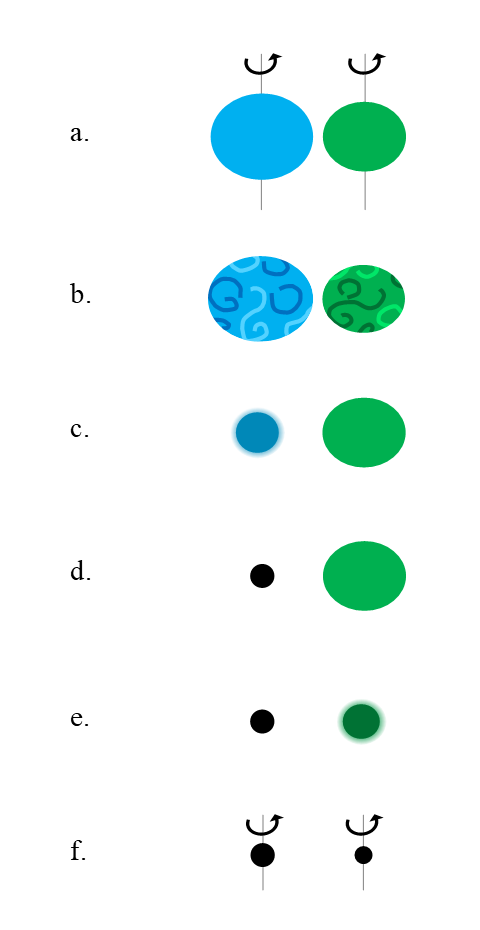
\includegraphics[width=0.4\textwidth]{channel2.png}
	\caption{\label{fig:chem_homog} A sketch of merging black\ilya{-}hole binary formation via the chemically homogeneous evolution channel.}
\end{figure}

What if some types of massive stars did not expand and converted most of their mass into a black hole? A massive binary could then start out at an orbital period of a couple of days, close enough that if the stars produced black holes in situ they would merge within the age of the Universe through gravitational-wave emission. Without an expansion phase, the parent stars would be in no danger of merger; if almost all of the star's mass was converted into a black hole rather than the $\sim$30--50\% of the mass which typically becomes the helium core (see \autoref{fig:BHremnant}), the merger timescale would shrink for a given separation, lifting the Roche lobe radius curve in \autoref{fig:Rmax} and removing the ``separation problem at birth''.  No fine-tuning of binary evolution would then be required to construct a plausible formation scenario for tight black-hole binaries.  This scenario does, however, require some unproven assumptions regarding stellar evolution. But it may be the case that high-mass, low-metallicity stars in close binaries behave exactly as needed for this scenario to work.

This evolutionary pathway is sketched out in \autoref{fig:chem_homog}:
\begin{itemize}
\item[a.] Binary companions raise tides on each other, much like the Moon's tides on Earth.  If a binary is tight enough that each star fills a significant fraction of its Roche lobe, tidal energy dissipation is rapid and proceeds until the stars are tidally locked, i.e. the rotation periods of the stars are synchronized to the orbital period of the binary. This also means that the stars are rotating at a few tens of percent of their break-up velocities.  
\item[b.] Such rapidly rotating stars will develop significant temperature gradients between the poles and the equator, which may lead to efficient large-scale meridional circulation within each star \citep{Eddington:1925,Sweet:1950}.  \citet{EndalSofia:1978} and subsequent studies \citep[e.g.,][]{Heger:2000,MaederMeynet:2000,Yoon:2006,Szecsi:2015} explored the internal shears and their impact on the mixing of chemical species within the star.  Although quantitative predictions differ, it appears that rapidly rotating massive stars may efficiently transport hydrogen into the core and helium out into the envelope until nearly all of the hydrogen in the star is fused into helium.  
\item[c--f.] Then, at the end of the main sequence, the star behaves essentially as a Wolf-Rayet naked helium star, contracting rather than expanding. As long as the metallicity is sufficiently low that the wind-driven mass loss does not significantly widen the binary -- which would lead to the loss of co-rotation and chemically homogeneous evolution \citep{deMink:2009} -- the binary can avoid mass transfer.  
\end{itemize}

\citet{MandeldeMink:2016,deMinkMandel:2016}, and \citet{Marchant:2016} explored such binaries and concluded that they could present a viable channel for forming the most massive observed gravitational-wave sources (such as GW150914), though not the lowest-mass systems.  

\subsubsection{The black\ilya{-}hole matchmaking club: dynamical formation in dense stellar environments}

\begin{figure}
	\centering
	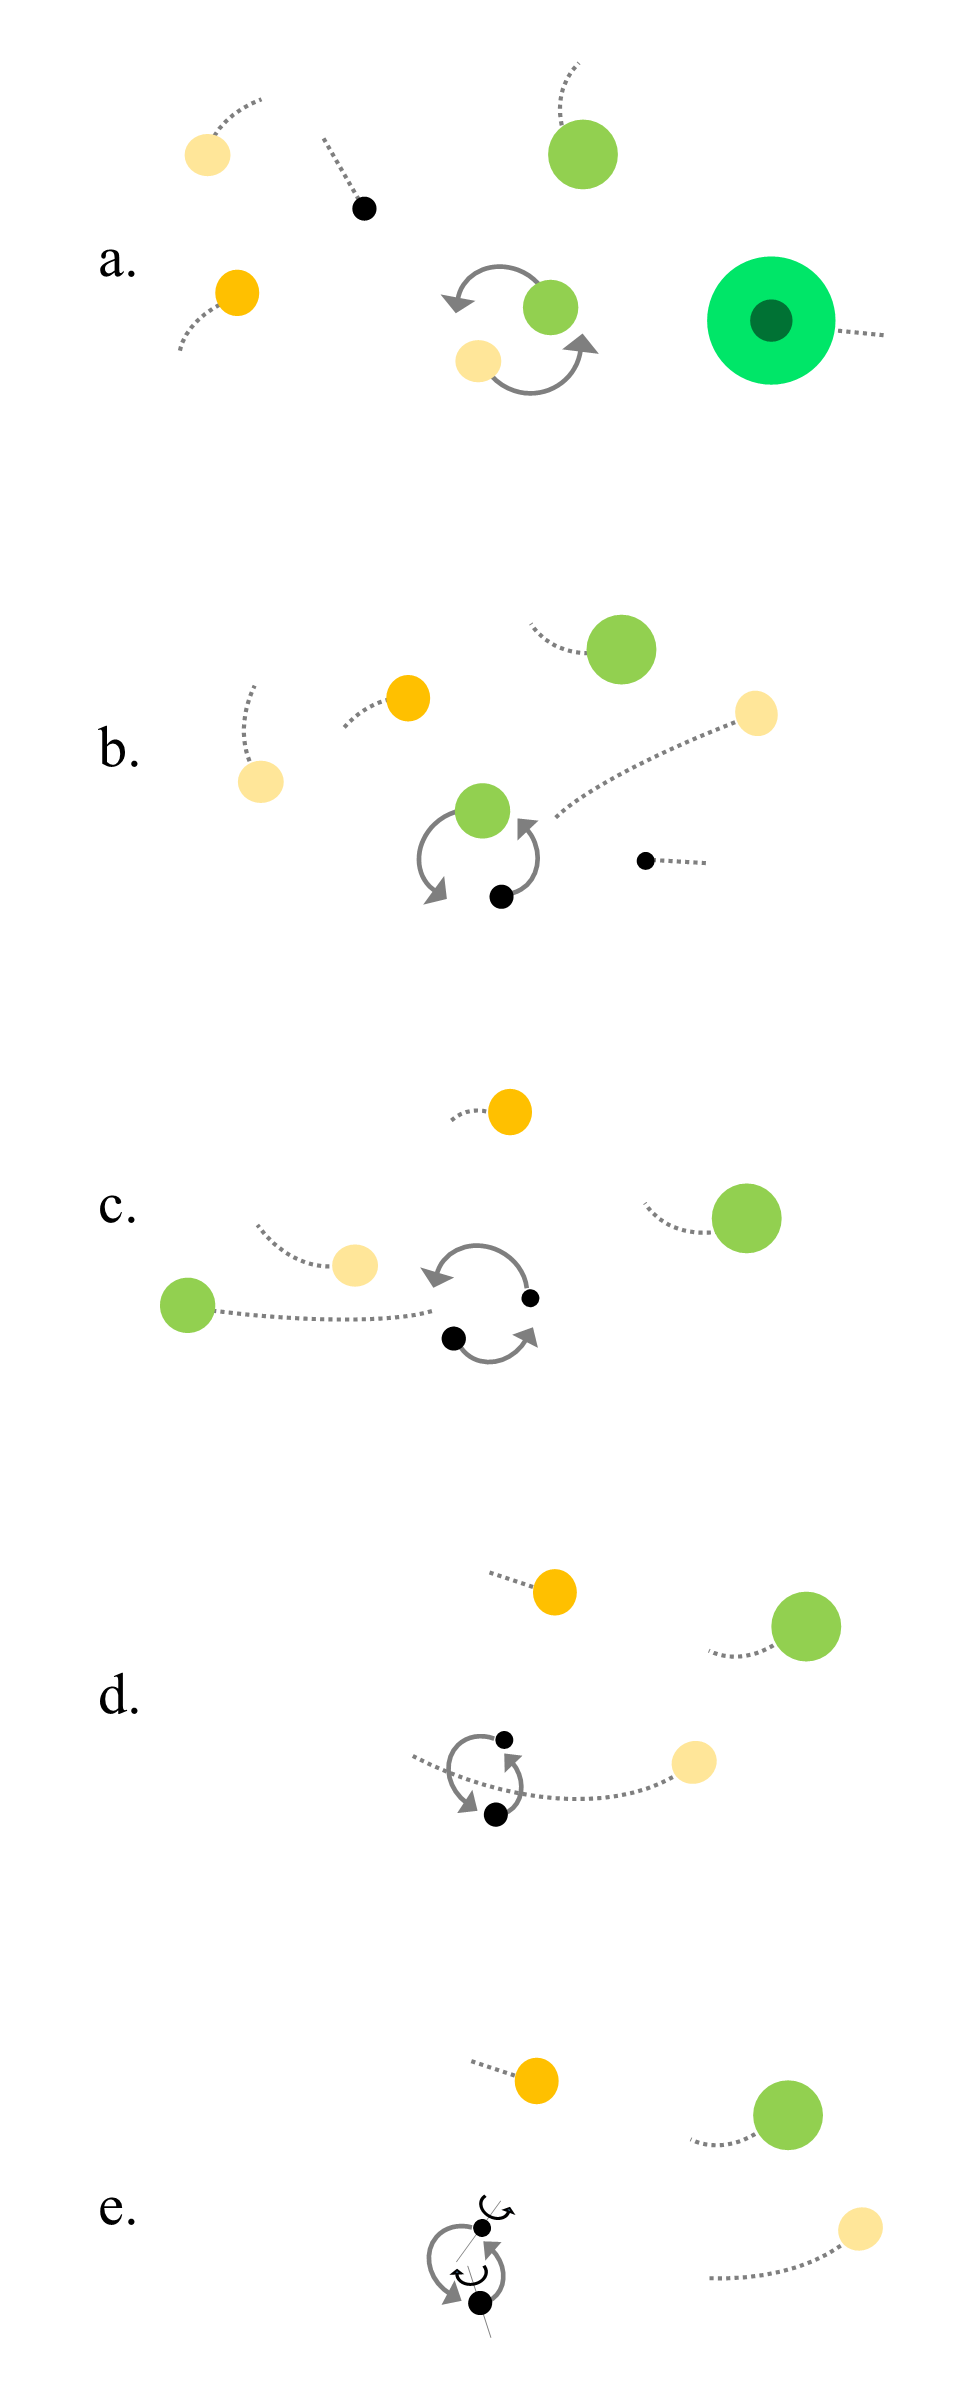
\includegraphics[width=0.4\textwidth]{channel3.png}
	\caption{\label{fig:dynamical} A sketch of merging black\ilya{-}hole binary formation via the dynamical evolution channel.}
\end{figure}

The last possibility we will describe is that the merging black holes may not have formed in the same binary at all.  Instead they formed from the collapse of independent massive stars (perhaps single, or each in its own separate binary), but were then introduced to each other by a matchmaker, or rather a whole array of matchmakers.   This evolution is illustrated in \autoref{fig:dynamical}: 
\begin{enumerate}
\item[a.] Suppose the two black holes formed in a dense stellar environment such as a globular cluster.  
\item[b.] As the most massive objects in the cluster, the black holes naturally sink toward the cluster center as energy is equipartitioned throughout the cluster in the process known as mass segregation \citep[but see][]{Trenti:2013}.  Once there, they may form binaries through three-body interactions, or by substituting into existing binaries: in a $2+1$ interaction, the lightest object is usually ejected in favor of the two heavier objects forming a binary.  
\item[c,d.] If the orbital speed of the binary's components is greater than the typical speed of stars in the cluster (the binary is `hard'), then subsequent interactions with other objects in the cluster -- the matchmakers -- will gradually tighten the black-hole binary. The interlopers are likely to leave with slightly higher speeds than they arrived with, each time removing energy from the binary.   Meanwhile, `soft' binaries, with orbital speeds smaller than the velocity dispersion in the cluster, will be disrupted.
\item[e.] If the density of objects is high enough to ensure a suitable rate of interactions, the binary will be hardened until it is compact enough to merge through gravitational-wave emission, provided it does not get kicked out of the cluster through a recoil kick from the last interaction -- and even then, it may still go on to merge outside of the cluster.  
\end{enumerate}

The prospects for these dynamically formed merging binary black holes in globular clusters and young massive stellar clusters have been explored through a series of analytical estimates and numerical experiments by \citet{Sigurdsson:1993,Kulkarni:1993,PZwart:2000,OLeary:2006,Banerjee:2010,Downing:2011,Morscher:2015,Mapelli:2016,Rodriguez:2016} and others.  \citet{OLeary:2008} \citep[but see][]{Tsang:2013} and \citet{AntoniniPerets:2012} explored dynamical formation in galactic nuclei with a massive black hole, while \citet{MillerLauburg:2008} and \citet{AntoniniRasio:2016} argued that galactic nuclei without a massive black hole are a favored site for dynamical formation, in part because the high escape velocity makes merger products more likely to be retained.  \citet{Bartos:2016} and \citet{Stone:2016} have described the role that an accretion disk in an active galactic nucleus could play in enhancing the rate of binary black hole mergers.

\subsubsection{A team effort: combining multiple interactions}

Of course, the channels outlined above need not be distinct, and the same binary may have benefited from multiple types of interaction while en route to coalescence.   \ilya{Studies that consistently combine stellar and binary evolution and dynamics at the same level of fidelity are scarce}.  Black holes brought together by dynamical interaction in globular clusters may be part of mass-transferring binaries earlier in their evolutionary histories.  Mass-transferring binaries that are too wide at the end of binary evolution to merge in the age of the Universe may be helped along by subsequent dynamical encounters \citep[e.g.,][]{Belczynski:2014VMS}.  The more massive star in an isolated binary may evolve chemically homogeneously, while its less massive companion expands and donates mass \citep{Marchant:2017}.  

Hierarchical triple systems, with a tight inner binary and a third companion on a wider outer orbit are a particularly promising combination of the isolated evolution and dynamical formation channels.  A significant fraction of massive stars appear to be born in triples and higher multiplicity systems \citep{DucheneKraus:2013}.  Triples may also be formed dynamically through binary--binary scatterings \citep{MillerHamilton:2002b}.  Massive black holes in galactic nuclei --- or intermediate-mass black holes in globular clusters --- may also act as effective triple companions.   

When the outer binary's orbit is $\gtrsim 5$ times wider than the inner orbit, the triple will be stable (though it may still be driven to instability by mass loss \citep[e.g.,][]{PeretsKratter:2012}).  If the inner and outer orbits in a stable triple have a high relative inclination angle, the transfer of angular momentum between these orbits can increase the eccentricity of the inner binary while keeping its semi-major axis roughly constant. For suitable initial conditions, these Lidov-Kozai oscillations in eccentricity and orbital inclination \citep{Lidov:1962,Kozai:1962} may lead to a drastic growth in the inner binary's eccentricity \citep[for a review, see][]{Naoz:2016}, reducing the binary's periapsis to the point where gravitational-wave emission can harden the binary to merger.  Recent arguments that Lidov-Kozai cycles could contribute to binary black hole mergers include \citet{SilbeeTremaine:2017} who explored isolated triples, \citet{Antonini:2016} in the context of dynamically formed triples in globular clusters, and \citet{Hoang:2018} who considered triples with a galactic-center massive black hole as the outer companion.


\section{Expected properties of merging systems}\label{merge}

In this section we describe the expected hallmarks of each formation scenario in the properties of observed binary black hole mergers. These properties include merger rates, black\ilya{-}hole masses, mass ratios, spins, orbital eccentricities, and formation environments.

Other than the LIGO and Virgo sources, there are no known direct observations of binary black holes (except for a very speculative potential observation through microlensing \citep{Dong:2007}). As the population of gravitational-wave detections grows, so will our ability to infer merger rates and typical system properties from observed data; see the following section for a discussion of the current state of these efforts. In the meantime, our understanding of the expected merger rates and properties of binary black holes rests largely on theoretical modeling. 

For the isolated binary evolution channel (\autoref{form:isol}) this modeling typically uses a population synthesis approach, i.e. forward modeling of large populations of stellar binaries distributed according to observed initial mass and separation distributions, some (small) fraction of which end up as merging binary black holes. Population synthesis techniques can be applied either to initial binaries at formation, or to specific observed systems at intermediate evolutionary stages, such as Cygnus X-1 \citep{Bulik:2008} and Cygnus X-3 \citep{CygnusX3:2012}.  

Models of the dynamical formation channel are typically based on either (i) computationally expensive N-body cluster models with direct integration of the equations of motion for each object, or (ii) a less computationally costly Monte Carlo approach in which the evolution of the distribution of the cluster components in phase space is coupled with stochastically sampled strong 3-body and 4-body interactions modeled with few-body dynamics, or (iii) semi-analytical prescriptions that attempt to emulate these methods at a fraction of the computational cost. 

\subsection{Merger rates}

Here we outline high-level estimates of merger rates for each of the three candidate formation channels. The value of this back-of-the-envelope merger rate analysis is not so much in matching the rate inferred from gravitational-wave observations a posteriori as in setting the stage for some of the predictions of the properties of merging binaries (see below) and the discussion of evolutionary uncertainties (see \autoref{prospect}).  That said, the merger rate predictions for isolated binary evolution via the common envelope phase are consistent with the observed rate of binary black hole mergers of around $\sim 10$ to $\sim 200$ Gpc$^{-3}$ yr$^{-1}$ \citep{GW150914:rates,GW170104} (see \citet{ratesdoc} for a slightly dated summary \ilya{-- the current estimates fall within the range of early predictions, at their upper end}); \ilya{predicted} dynamical formation rates tend toward the lower end of this range \citep{Rodriguez:2016,Park:2017,FragioneKocsis:2018}; and chemically homogeneous evolution could yield tens of \ilya{high-mass} mergers per Gpc$^{3}$ per yr$^{-1}$ in the local Universe \citep{MandeldeMink:2016,Marchant:2016}.

\subsubsection{Binary evolution via a common envelope}\label{sec:CErates}

In order to survive an evolutionary pathway such as the one depicted in \autoref{fig:isol_binary}, a binary must (i) have the right component masses to form two black holes; (ii) have the right separation to avoid a premature merger, yet be close enough to interact; (iii) avoid disruption by supernova kicks; (iv) engage in and survive a common envelope phase; and (v) end up sufficiently compact at binary black hole formation to merge within the age of the Universe. We describe below the development of a ``Drake equation'' for the probability that an isolated stellar binary will end its life as a merging binary black hole, addressing each of these five factors in turn.   In reality, of course, the probabilities for each key stage are coupled in a rather complex manner.

\begin{enumerate}
	\item[(i)] The minimal initial stellar mass for forming a black hole is likely around $20 M_\odot$, so $f_\textrm{primary} \approx 0.1\%$ of all stars drawn from the \citet{Kroupa:2002} initial mass function will form black holes. Although this can be shifted somewhat by binary interactions, we will use this approximation for the purpose of this back-of-the-envelope calculation. Meanwhile, since the mass ratio between the primary and the secondary is roughly uniformly distributed \citep{Sana:2012,MoeDiStefano:2017}, roughly half of the secondaries will fall into the mass range of interest, $f_\textrm{secondary} \approx 0.5$.  

\item[(ii)] Initial binary  separations are observed to be distributed uniformly in the logarithm, $p(a) \propto 1/a$ \citep{Opik:1924}.  The first episode of mass transfer from the donor should typically be ``case B'' mass transfer (i.e., the donor should evolve beyond core hydrogen burning, but not yet beyond core helium burning); stars expand by several orders of magnitude during this phase, which means that the range of initial separations occupies a significant logarithmic fraction of the total initial range of separations, so $f_\textrm{init sep} \approx 0.5$.  

\item[(iii)]  We assume that black holes receive low natal kicks and do not lose significant amounts of mass, so that supernovae do not significantly affect binary parameters, i.e. $f_\textrm{survive SN1} \approx f_\textrm{survive SN2} \approx 1$.  

\item[(iv)] The fraction of binaries that initiate and survive the common envelope phase during mass transfer from the secondary to the primary is perhaps the least certain.  Typically, dynamically unstable mass transfer is more likely for greater mass ratios of the donor to the accretor.  The accreting black hole in this case may only have a third of the initial mass of the primary, with the rest lost with the envelope and through winds, while the secondary donor may have increased its mass during the first mass transfer phase; even so, unless the secondary was initially close to the primary in mass, the mass ratio is unlikely to exceed $3:1$, which may be close to the threshold for initiating a common envelope phase.  The evolutionary state of the donor during the onset of mass transfer also plays an important role, setting both the amount by which the donor shrinks or expands in response to mass loss and the envelope binding energy.  Together, these constraints reduce the fraction of successful common envelope initiations and ejections to $f_\textrm{CE} \approx 0.1$.  

\item[(v)]  Finally, there is the question of final separation at second black hole formation, as only systems with separations smaller than those in \autoref{fig:periapsis} will merge in the age of the Universe.  The final separation after the common envelope ejection is set by the binding energy of the envelope at the time when the secondary initiates unstable mass transfer, which in turn depends on the binary separation at that time.  Therefore, very crudely, the flat-in-the-log distribution of initial binary separations persists to the final binary separation.  Since the delay time between formation and merger $\tau_\textrm{GW} \propto a^4$ is a power law in the separation, the delay time distribution also follows a flat-in-the-log distribution $p(\tau) \propto 1/\tau$.  Among the binaries that survive a common envelope the closest will be those whose separations just barely encompass a Wolf-Rayet star, i.e., with separations of a few solar radii (and merger times of a few million years).  The logarithmic distribution ensures that tens of percent of binaries that survive a common envelope will merge in the age of the Universe, $f_\textrm{merge} \approx 0.2$.
\end{enumerate}

Thus, our Drake\ilya{-like} equation is as follows:
\begin{eqnarray}
f_\textrm{BBH} &=& f_\textrm{primary} \times f_\textrm{secondary} \times f_\textrm{init sep} \times f_\textrm{survive SN1} \times f_\textrm{CE} \times f_\textrm{survive SN2} \times f_\textrm{merge} \nonumber \\
 & \sim & 0.001 \times 0.5 \times 0.5 \times 1 \times 0.1 \times 1 \times 0.2 = 5 \times 10^{-6}.
\end{eqnarray}
Merging binary black holes are rare outcomes indeed!  [Merging binary neutron stars are similarly rare: while stars with initial masses sufficient to form a neutron star, between roughly 8 and 20 solar masses, are more common than the heavier stars necessary to form black holes, neutron star natal kicks and mass loss during supernovae are more likely to disrupt binaries; the expected yields for binary neutron star mergers are within an order of magnitude of those for binary black holes.]

The star formation rate in the local Universe is $\sim 0.01 M_\odot$ Mpc$^{-3}$ yr$^{-1}$ \citep{MadauDickinson:2014}; for an average binary mass of $\sim 1 M_\odot$, the yield $f_\textrm{BBH} \sim 5 \times 10^{-6}$ corresponds to a binary black hole merger rate of $\sim 50$ Gpc$^{-3}$ yr$^{-1}$, or 5 per Myr for a Milky-Way equivalent galaxy with a space density of $0.01$ Mpc$^{-3}$.  Of course, the actual calculation of the binary merger rate requires significantly more care than the back-of-the-envelope model presented here, including accounting for the redshift-dependent metallicity-specific star formation history convolved with the time-delay distribution.  

\subsubsection{Chemically homogeneous evolution}

We can write a similar Drake's equation for the chemically homogeneous evolution channel.  Following \citet{MandeldeMink:2016},  the yield fraction is
\begin{eqnarray}
f_\textrm{BBH} &=& f_\textrm{primary} \times f_\textrm{secondary} \times f_\textrm{init sep} \times f_Z \times f_\textrm{merge} \nonumber \\
 & \sim & 0.0002 \times 0.5 \times 0.1 \times 0.1 \times 1 = 10^{-6}.
\end{eqnarray}

Here, $f_\textrm{primary} \approx 2 \times 10^{-4}$, lower than the value in the previous paragraph because only the most massive stars with initial masses above $\sim 50 M_\odot$ are likely to have the necessary level of mixing to undergo chemically homogeneous evolution; and $f_\textrm{secondary} \approx 0.5$ as above.  In order to engage in efficient mixing, the components must be close enough to be tidally locked and rotating at a significant fraction of the break-up velocity, yet avoid merger; this defines a range of initial separations spanning roughly a factor of 2 out of a total range spanning $\approx 5$ orders of magnitude, so $f_\textrm{init sep} \approx 0.1$ assuming a flat-in-the-logarithm distribution of initial separations.  Finally, $f_Z \approx 0.1$ is the total historical fraction of low-metallicity star formation, required to suppress line-driven winds which widen the binary, spin down the stars, and suppress mixing.  Because these binaries are constructed to be very tight at birth, the vast majority should merge after the stars collapse into black holes in situ, and $f_\textrm{merge} \approx 1$. Thus, if this channel is viable, the rate of binary black hole mergers produced through the chemically homogeneous evolution channel could reach perhaps $\sim 10$ Gpc$^{-3}$ yr$^{-1}$, but with a preference for much higher masses than classical isolated binary evolution.


\subsubsection{Dynamical formation}

We can estimate an upper limit on the merger rate of dynamically formed binary black holes by assuming that all black holes in a globular cluster undergo a single merger.  About 1 in a thousand stars are massive enough to become a black hole ($f_\textrm{primary} \approx 0.001$), so even a relatively large cluster with $2\times 10^6$ stars would produce \ilya{at most} 2000 black holes and 1000 mergers.  [Although repeated mergers are possible if the black hole merger product is retained in the cluster and merges again, they are very rare as gravitational-wave recoil kicks are overwhelmingly likely to eject a merger remnant from the cluster \citep{Rodriguez:2018}; in any case, even merging all black holes sequentially would increase this estimate by at most a factor of 2.]  If we imagine that the merger rate is uniform over the $\sim 10$-Gyr history of the Universe (if mergers predominantly happened early in the cluster history, the rate in the local Universe would be lower), and with a globular cluster space density of around 1 per Mpc$^3$, the {\it upper limit} on the merger rate from this channel is $\sim 1000 \times 10^{-10} \textrm{yr}^{-1} \times 1 \textrm{ Mpc}^{-3} \approx 100$ Gpc$^{-3}$ yr$^{-1}$.

Young massive star clusters could add to this rate \citep[e.g.,][]{Ziosi:2014}, as could galactic nuclear clusters \citep[e.g.,][]{MillerLauburg:2008,Bartos:2016,Stone:2016,AntoniniRasio:2016}.  On the other hand, in practice, the overall merger rate from the dynamical formation channel is likely to be at least a factor of a few lower for the following reasons:
\begin{enumerate}
	\item [1.]
Some single black holes will be ejected from the cluster during the three-body interactions that harden the binaries.  If the masses of all interacting objects are similar, the ejected object receives a kick that is comparable to the orbital speed of the binary.  The last scattering interaction must harden the binary to a sufficiently small separation for gravitational-wave emission to take over. The minimum orbital velocity of an equal-mass circular binary that can merge in the age of the Universe through gravitational-wave emission is $\sim 200$ km s$^{-1}$; this scales only weakly with the binary's mass, as $v \propto \sqrt{M/a}  \propto \sqrt{M/M^{3/4}} \propto M^{1/8}$ (see \autoref{fig:periapsis} and \citet{Peters:1964}).   This minimum velocity is larger than the typical globular cluster escape velocity, $\lesssim 50$ km s$^{-1}$, hence many interlopers, including some black holes, will be ejected.
	\item[2.]
Following such a 3-body interaction, the binary itself must recoil in the opposite direction from the ejected single star (to conserve momentum). Although this recoil velocity is reduced by the ratio of the binary's mass to the interloper mass --- typically greater than $2:1$, as the lightest body is ejected --- the binary may still be ejected from the cluster before it is sufficiently tight to merge through radiation reaction alone.
\item[3.] If most mergers happen soon after globular cluster formation, the local merger rate would be low because the majority of globular clusters are old \citep{Rodriguez:2016big}.
\end{enumerate} 

\subsection{System Properties}
\subsubsection{Masses}
The masses of black holes in the binaries of interest will not change appreciably after the black holes are formed by stellar collapse or supernova explosions.  The first black hole to form is unlikely to accrete a significant amount of mass from its companion: doubling its mass would take more than 100 million years, as the mass-gain rate is $\dot{M}/M \lesssim 10^{-8}$ yr$^{-1}$ at the Eddington limit, and the massive companion will only survive as a non-degenerate potential donor star for a small fraction of that time. No further accretion is expected in the system after the second compact object is formed. The mass of each black hole is thus almost equal to its mass at formation. 

The classical isolated binary evolution channel can produce binary black holes with a broad range of masses, matching all observations to date \citep[e.g.,][]{Stevenson:2017,Eldridge:2017,GiacobboMapelli:2018} as well as GW170817 and the observed Galactic double neutron stars \citep[e.g.,][]{Kruckow:2018,VignaGomez:2018}.  In fact, contrary to mistaken lore, the high masses of the first observed black holes were not entirely surprising: such systems were predicted to arise in low-metallicity environments, and to make a significant contribution to the detected population because more massive binaries emit more energy in gravitational waves \citep{Dominik:2014}; the effect of metallicity is discussed further in \autoref{environ} below. 

Dynamical formation in globular clusters can also lead to a range of masses, but may favor more massive binaries: lighter black holes would be ejected by heavier ones in three-body interactions \citep{Rodriguez:2015}. The mass distribution is sensitive to natal kicks, which may eject black holes at formation \citep{Zevin:2017}.  \citet{Chatterjee:2017} argue that dynamical formation could explain all black\ilya{-}hole binary merger observations to date, with old, metal-poor clusters preferentially contributing more massive black\ilya{-}hole binaries and younger, metal-rich clusters contributing lighter binaries.
 
Chemically homogeneous evolution can only produce massive binaries, with total black\ilya{-}hole mass above $\sim 50 M_\odot$ \citep{MandeldeMink:2016,Marchant:2016}.

\subsubsection{Mass ratios}
The mass ratios of merging black\ilya{-}hole binaries produced through the isolated binary evolution channel are likely to be on the equal side of $2:1$, because of the mass ratio constraints necessary to ensure stable mass transfer from the primary to the secondary and then dynamically unstable reverse mass transfer. However, mass ratios exceeding $2:1$ are expected to be more common at low metallicity \citep{Dominik:2012,Stevenson:2017}.

Dynamically formed binaries may also favor comparable masses because the heaviest black holes in a cluster are most likely to merge, though more extreme mass ratios are also possible if the globular cluster contains a particularly heavy stellar-mass black hole or a $\gtrsim 100 M_\odot$ intermediate-mass black hole \citep{Mandel:2008,Belczynski:2014VMS}. 

Chemically homogeneous evolution has a much stronger preference for equal masses \citep{MandeldeMink:2016}.  \citet{Marchant:2016} concluded that nearly equal-mass black holes would be produced from the evolution of systems that were in contact (shared mass) on the main sequence, before disengaging during subsequent phases of chemically homogeneous evolution and proceeding along the pathway sketched out in \autoref{sec:CHE}. 

\subsubsection{Black\ilya{-}hole spin magnitudes and directions}\label{BHspins}
The spins of merging black holes may carry imprints of their evolutionary history. 

Isolated binaries, including those formed through chemically homogeneous evolution, are generally expected to have preferentially aligned spins after undergoing episodes of mass transfer and/or tidal coupling, although natal kicks and possible spin tilts during supernovae could lead to misalignment \citep[e.g.,][]{Farr:2011,Tauris:2017}.  Meanwhile, the spin directions for dynamically formed binaries are likely to be distributed isotropically \citep[e.g.,][]{Rodriguez:2016spin}.  On the other hand, black holes merging through the Lidov-Kozai resonance in hierarchical triples could preferentially have spins in the orbital plane \citep{LiuLai:2018,RodriguezAntonini:2018}.

Spin magnitudes may also depend sensitively on evolutionary history.  A massive star may contain a large amount of angular momentum, far in excess of the maximum allowed for a spinning black hole. However, the vast majority of that angular momentum will be contained in the outer layers of the star and can therefore readily be lost through winds or via envelope stripping by a companion.  Therefore, black holes formed from stars that were rapidly spinning at some point in their evolution may still spin slowly unless the stars are spun up through mass transfer or tides shortly before collapse \citep{Kushnir:2016,HotokezakaPiran:2017,Zaldarriaga:2017} or during the supernova itself \citep{Batta:2017,Schroeder:2018}.   This argument for slowly spinning black holes in compact binaries is potentially in conflict with the claimed observations of rapid spins in black-hole high mass X-ray binaries \citep{MillerMiller:2015}.     However, the spin magnitude measurements in X-ray binaries could be very sensitive to the modeling assumptions, and the systematic errors may dominate the statistical ones \citep[e.g.,][]{Basak:2017,Kawano:2017}. Moreover, there may be significant differences in the evolutionary channels and environments of the locally observed high-mass X-ray binaries and the binary black holes observed in gravitational waves \citep[][and see \autoref{environ}]{HotokezakaPiran:2017}.

Gravitational-wave spin measurements have so far only constrained the effective spin, which enters the phasing of gravitational waves at the 1.5 post-Newtonian order \citep{PoissonWill:1995}.  The low effective spins of the first four detected merging black holes allowed \citet{Farr:2017} to conclude that either the spin directions were isotropically distributed or the spin magnitudes were low.

\subsubsection{Orbital eccentricities}
	The orbital eccentricities of merging black\ilya{-}hole binaries may contain information about their past \citep{MandelOShaughnessy:2010}. Because gravitational waves are very efficient at damping out orbital eccentricity, isolated binaries are expected to merge on circular orbits. Dynamically formed systems may, however, retain detectable eccentricities at merger if their orbits are very tight at formation: the periapsis of a highly eccentric binary would need to be $\lesssim 10^4$ km in order for the eccentricity to exceed 0.1 when the gravitational-wave frequency reaches the minimum of the detector sensitivity band at 10 Hz.  Dynamical formation of very tight binaries may be possible through two-body captures in Galactic nuclei \citep{OLeary:2008} \citep[but see][]{Tsang:2013}; in some hierarchical triples evolving through the Lidov-Kozai mechanism \citep[e.g.,][]{AntoniniPerets:2012}; or through close captures during three-body interactions \citep{Samsing:2014, Rodriguez:2018}. 


\subsubsection{Formation environments}
\label{environ}
The evolutionary history of merging black holes is also dependent on their formation environments, particularly through the effect of chemical composition (metallicity) on stellar evolution and thereby black\ilya{-}hole mass.

Black\ilya{-}hole masses are set by the mass of the parent star at the end of stellar evolution, preceding the collapse or supernova explosion, and by the amount of ejecta during the supernova. Observational evidence and collapse models suggest that sufficiently massive stellar cores may completely collapse into black holes \citep[for a review, see][]{Mirabel:2016}. Thus, the mass of the stellar core --- the convective region in the center of the star where nuclear fusion proceeds from hydrogen through helium, carbon, oxygen, and so on to iron --- determines the ultimate black\ilya{-}hole mass.  If left unperturbed, of order a third of the mass of a massive star will end up in a carbon--oxygen core, and thereby in the black\ilya{-}hole remnant.

The intense radiation from massive stars with luminosities $\sim 10^5 L_\odot$ drives significant winds, which can remove a large amount of material from the star. The mass of the star at the end of stellar evolution can thus be much lower than the star's initial mass, and the mass of the resulting compact object can therefore be much lower than $1/3$ of the initial stellar mass. Metals like iron, with their many absorption lines, are particularly efficient at capturing the stellar radiation and transforming it into outward momentum.  Therefore, the metal fraction, or metallicity  --- the fraction $Z$ of the star's mass contained in elements heavier than hydrogen and helium --- is a key ingredient in determining stellar wind mass loss rates \citep{Vink:2001}. Although wind models are uncertain \citep[e.g.,][]{Renzo:2017}, simulations suggest that at the 2\% metallicity of our solar neighborhood, massive stars lose enough mass via winds that maximum black\ilya{-}hole masses are only around $15 M_\odot$ \citep{Belczynski:2009,Spera:2015}. This matches the masses of black holes observed in X-ray binaries. Figure \ref{fig:BHremnant} illustrates the dependence of compact remnant mass on metallicity. 
 
\begin{figure}
	\centering
	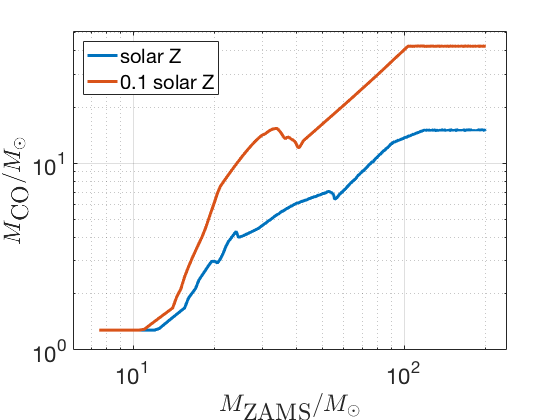
\includegraphics[width=0.5\textwidth]{BHremnantdelayed.png}
	\caption{\label{fig:BHremnant} Remnant compact object mass from single stellar evolution for a given zero-age main sequence stellar mass, following the default COMPAS prescription for winds \citep{Stevenson:2017}  and the `delayed' \citet{Fryer:2012} supernova fallback prescription, at solar ($Z_\odot=0.02$) metallicity (blue) and a tenth solar (red).  COMPAS sets a compact object mass threshold of $2.5 M_\odot$ between neutron stars and black holes.
	} 
\end{figure}

Forming heavier black holes, like those observed through gravitational waves, requires stellar progenitors born in regions with lower metallicity. The yield of merging black holes per unit star-forming mass is also greatest at lowest metallicity, due largely to the reduced wind-driven mass loss \citep[e.g.,][]{Belczynski:2010,Kruckow:2018}. For the isolated binary channel, delayed stellar expansion at lower metallicity, which allows the stars to develop a larger helium core before engaging in mass transfer, further enhances this effect \citep[e.g.,][]{Stevenson:2017}.

The above considerations place constraints on the formation time of the systems that produced the observed merging black\ilya{-}hole binaries. Most low-metallicity star formation occurred in the early Universe, before the interstellar medium was polluted with metal-rich products of stellar evolution; however, a broad range of stellar metallicities is observed at all epochs  \citep[e.g.,][]{LangerNorman:2006,TaylorKobayashi:2015}. Meanwhile, population synthesis models of the classical formation channel indicate that the distribution of delay time $\tau$ between star formation and merger peaks at shorter delay times, with a $p(\tau) \propto 1/\tau$ decay.  This time delay distribution is consistent with gravitational-wave driven merger time scales for binary separations distributed as $p(a) \propto 1/a$ at the time of double black hole formation (see \autoref{sec:CErates}), but  is robust to moderate changes in separation distribution because of the very steep scaling of the delay time with separation, $\tau \propto a^4$.  (Other formation channels, particularly chemically homogeneous evolution, predict very different delay time distributions, potentially providing an additional way to discriminate between formation channels.)  A convolution of the metallicity-specific star formation history and the delay-time distribution led \citet{Belczynski:2016} to conclude that, a posteriori, there was a bimodal probability distribution on the formation time of the binary star progenitor of GW150914: it either formed in the first $\sim$ Gyr after the Big Bang, with a long subsequent delay to merger \citep{Dominik:2014}, or formed more recently in a low-metallicity region such as a low-mass satellite galaxy.  

  

\section{Prospects for gravitational-wave astronomy}\label{prospect}

The half dozen gravitational-wave events observed to date provide limited conclusive information about the astrophysics of binary black holes and their progenitors.  Fortunately, these observations indicate a binary black hole merger rate of around $\sim 10$ to $\sim 200$ Gpc$^{-3}$ yr$^{-1}$ \citep{GW150914:rates,GW170104}, which points to the prospect of a few tens of detections in the next observing run and hundreds within the next three years, once the LIGO and Virgo instruments reach design sensitivity \citep{scenarios}.  This will yield enough information about both individually exciting events and population distributions to inaugurate gravitational-wave astronomy as a genuine tool for exploring stellar and binary evolution.  In this section, we describe some of the prospects for extracting information from the growing data set of observations over the next few years, including single informative observations, population statistical inference, and theoretical modeling.

\subsection{Individual exciting events}
Single events that would be individually informative include the discovery of a merging binary black hole with a component mass in the pair-instability supernova mass gap.  Models of pair instability supernovae suggest that no black holes with masses between $\sim 60 M_\odot$ (possibly reduced to $\sim 45 M_\odot$ by pulsational pair instability \citep{Woosley:2017}) and $\sim 130 M_\odot$ should form as a result of stellar collapse, with black\ilya{-}hole formation possible only outside this mass gap \citep{Marchant:2016}.  Therefore, the discovery of a single object in this mass gap would point to either past dynamical mergers that left the merger remnant to be reused in a dense stellar environment \citep{Rodriguez:2018}, or to a theoretical failure in pair instability models. 

Similarly, the discovery of a merger component with a mass between $\sim 2.1 M_\odot$ and $\sim 4.5 M_\odot$, in the range between the most massive known neutron stars and least massive black holes \citep{Ozel:2010,Farr:2011} would shed light on supernova explosion models, specifically the amount of fallback that can occur before the explosion \citep{Fryer:2012}.

Other individually exciting events could include the first confirmed discovery of an intermediate-mass black hole in the few-hundred solar-mass range, either as a merger of two such black holes \citep[e.g.,][]{AmaroSeoaneSantamaria:2009,Veitch:2015,Graff:2015} or as an intermediate-mass-ratio inspiral of a stellar-mass compact object into such a black hole \citep[e.g.,][]{Mandel:2008,Haster:2015IMRI,Haster:2016}. 

A source with a detectable eccentricity would clearly signal a dynamical capture \citep{Breivik:2016}. 

A measurement of an effective spin value close to either 1 or $-1$ would point to rapid spins of both black holes. A substantial positive effective spin coupled with high masses would point to the likelihood of chemically homogeneous formation \citep{Marchant:2016}, while a substantially negative effective spin measurement would indicate an unexpected anti-alignment between rapid spins and the binary's orbital angular momentum, perhaps through either a supernova spin tilt or dynamical formation.  

Although electromagnetic transients are not broadly expected to be associated with binary black hole mergers \citep[e.g.,][]{Lyutikov:2016}, any such observations would indicate the persistence of material around the merging binary \citep[e.g.,][]{deMinkKing:2017}.

\subsection{Population statistics}

Population statistics will generally yield more information than individual events.  We can use the statistical analysis of sufficiently large observational data sets to infer bulk properties of the source population, such as the mass and spin distributions, and to search for distinct subpopulations.  We can separate the approaches to inference on the observed populations into two types: unmodeled or weakly modeled inference, and inference that relies on \ilya{specific} accurate models. 

At the most basic end of weakly modeled inference is the (possibly non-parametric) reconstruction of an underlying distribution, such as the mass function of merging black holes \citep{Mandel:2010stat,BBH:O1}, while accounting for measurement uncertainties and selection effects.  For example, \citet{Fishbach:2017mass} use a weakly parametrized model to argue for the possible evidence of a mass gap due to pair-instability supernovae, while \citet{TalbotThrane:2017} discuss weakly parametrized inference on the spin distributions.  Meanwhile, the time delay between star formation and binary merger could be extracted by comparing the merger rate as a function of redshift against the star formation rate as a function of redshift \citep{Mandel:2016select}.  

We can look for distinct subpopulations or ``clusters'' of events in the observable parameter space, in the hope of finding distinct categories corresponding to different evolutionary channels.  \citet{Mandel:2015} argued that $\sim 60$ observations would make it possible to determine whether there are distinct subpopulations of events in mass space even after allowing for the significant measurement uncertainties inherent in gravitational-wave astronomy, and \citet{Mandel:2016cluster} demonstrated the feasibility of a particular clustering technique.  Meanwhile, \citet{Farr:2018} propose classifying binary black hole mergers by spin misalignment angle into aligned and isotropically distributed subpopulations.  It is worth noting that such clustering or classification schemes cannot hope to correctly assign individual events to a specific cluster: this is generally impossible given the significant measurement uncertainties \citep{Littenberg:2015}; instead, the goal is to measure the relative frequencies of events in different categories.

The next level of population-based inference relies on assuming that precise, possibly parametrized, subpopulation distributions are known.  In this case, hierarchical modeling \citep[extreme deconvolution in the language of][]{Hogg:2010} can be used to simultaneously determine the ratios of different subpopulations (e.g., arising from different formation channels) and any free parameters in the subpopulation models.  \citet{Zevin:2017} found that with $\sim 100$ observations, the mass distribution alone could be used to determine the formation channel, assuming the availability of trustworthy models of the mass distribution under different formation channels.  \citet{Vitale:2015} and \citet{Stevenson:2017spin} carry out a similar investigation for spin-orbit misalignment angles; although these cannot be measured with the same accuracy as chirp masses, several hundred observations should again be sufficient to distinguish multiple formation channels \ilya{and measure their branching ratios} through hierarchical modeling --- again, if the distributions under different channels are known \citep{Stevenson:2017spin}.  

\subsection{The future of population synthesis techniques}
There is, of course, a multitude of uncertain physics within any given model, both limiting the usefulness of approaches that rely on a precise knowledge of subpopulation distributions and, more importantly, providing a set of key science questions that we would like to answer with the aid of gravitational-wave observations.  How much mass do stars lose in winds, and what is the precise impact of metallicity and rotation on stellar evolution \citep[e.g.,][]{Renzo:2017}?  What happens to the star's angular momentum during collapse, how much mass is ejected, and how much of an asymmetric kick does the remnant receive \citep[e.g.,][]{Mirabel:2016}? How conservative is mass transfer in binaries, and how much angular momentum is carried away by the mass lost from the binary during non-conservative mass transfer \citep[e.g.,][]{vandenHeuvel:2017,Kruckow:2018}?  What are the conditions for the onset of a common-envelope phase and common envelope ejection, and how does the binary change in the process \citep[e.g.,][]{Ivanova:2013,Kruckow:2016}?   How do dynamical interactions affect binary evolution?  And, in turn, how do massive stellar binaries and their compact remnants feed back into astrophysics and cosmology on all scales?

One approach to addressing these big questions is to use the framework of population synthesis, which makes it possible to parametrize the uncertain physics and predict the expected source rates and distributions under different models.  Most efforts to date have relied on a discrete set of a few models in the parameter space of population synthesis assumptions \citep[e.g.,][]{Dominik:2012,Stevenson:2015}.  Even with the low computational cost of population synthesis, it is not feasible to explore more than a few tens to a few hundred models, and this is not sufficient to cover the full parameter space or to consider the correlations between model parameters.  However, recent successes in building accurate and computationally efficient emulators over the model parameter space \citep{Barrett:2017} suggest that a full exploration of this space will soon be possible. \citet{Barrett:2017FIM} applied Fisher information matrix techniques to the space of model parameters and found that parameters such as those describing mass loss rates during the Wolf-Rayet and luminous blue variable phases of evolution, and common\ilya{-}envelope energetics, can be measured to the level of a few percent with a thousand detections. 

\subsection{Other datasets and future missions}
Additional observational datasets will further aid in interpreting gravitational-wave observations and in refining models of binary stellar evolution.

Future gravitational-wave missions raise the prospect of observing the evolution of populations of merging binaries -- or individual systems -- across a broad band of frequencies, from the millihertz \citep[e.g.,][]{Sesana:2016} through the decihertz \citep{Mandel:2017} and hertz \citep{ET:2012}, to the LIGO/Virgo band.  The ability to track individual sources and source populations across the frequency spectrum will make it possible to combine information which can best be measured at low frequencies (e.g., eccentricity and sky location) and high frequencies (e.g., spins).  Meanwhile, a stochastic background of gravitational waves from individually unresolvable binary black holes could be measured in the next few years \citep{GW150914:stoch}, possibly providing additional insight on high-redshift populations; however, the only constraining parameter in a detection of such a background will likely be its amplitude, which carries only limited information \citep{Callister:2016}.

Ultimately, the most useful constraints are likely to come from the requirement that any candidate evolutionary model must self-consistently explain all of the available data: gravitational-wave observations, perhaps in multiple frequency bands, as well as electromagnetic observations of X-ray binaries, Galactic neutron stars, gamma ray bursts, supernovae, luminous red novae, etc. Incorporating these constraints will make it possible to resolve modeling degeneracies and to build a concordance model of massive binary evolution.  

\subsection{Outlook}

Today we have a half-dozen observations of merging binary black holes.  That is a half-dozen more than three years ago, and we have already learned a great deal.  Binary black holes exist. They merge. They do so relatively frequently.  They have a broad range of masses, and none of the sources seen so far seem to have rapid net spins in the direction of the orbital angular momentum.  We also have several plausible evolutionary channels, some of which appear to explain many of the observed properties (merger rates and masses). Black\ilya{-}hole spins continue to present something of a puzzle, particularly in light of the claimed high spins in a few high-mass black-hole X-ray binaries.

At the same time, we have the tools in place to create detailed models of stellar and binary evolution and of dynamical interactions under a variety of parameterizable assumptions.  The statistical techniques for analyzing the data and inferring properties directly from the observations, or by comparison with the detailed models, are in place.  Most importantly, we have wonderful detectors which are continuing to improve, and we expect to obtain enough data in the next few years to carry out these analyses.  Perhaps in a few years we will know that all of the channels described here contribute non-negligibly to binary black hole formation; that black holes receive small kicks at birth; and that they spin slowly in merging binaries. We may also have made the first detections of new objects such as $200 M_\odot$ intermediate-mass black holes.

The future of gravitational-wave astronomy holds the thrilling prospect of addressing the inverse problem of massive binary stellar evolution: inferring the formation channels and their physics from observations of the merging compact-object binary population.  Like a paleontologist who uses her knowledge of anatomy to determine the appearance, eating habits, and even behavior of extinct dinosaurs from their fossilized remnants, we can now use merging black holes --- remnants of massive stars --- to probe the behavior of those stars, and particularly their evolution in binaries.


\begin{acknowledgements}
We would like to thank Christopher Berry, Cole Miller, Fred Rasio, Dorottya Sz\'{e}csi, and Thomas Tauris for comments that significantly improved this manuscript, and Lev Yungelson and Ed van den Heuvel for providing a historical perspective.

IM is grateful to the students who contributed to building COMPAS (Jim Barrett, Sebastian Gaebel, Coenraad Neijssel, Simon Stevenson, Alejandro Vigna G\'{o}mez) and external collaborators (including Stephen Justham, Philipp Podsiadlowski, and especially Selma de Mink).  Coenraad Neijssel deserves additional gratitude for assistance with figures \ref{fig:Rmax} and \ref{fig:BHremnant}. Thanks also to  Will Farr, Vicky Kalogera and Gijs Nelemans for stimulating discussions spanning many years.

AF is grateful for the astro-tourism.
\end{acknowledgements}

\bibliographystyle{hapj}
\bibliography{Mandel}

\end{document}

Vicky: refs on p. 4 (list of other observables), 5 (XRBs and their discussion),  bottom of 6, 8, bottom of 9, top of 10, 16, 17, 18, check 19, 


